\chapter{Resultados parciais e Discuss\~{a}o}

Salvo menção contrária, os valores em porcentagem expressos neste capítulo se referem à base de cálculo em função da massa.

\section{Experimentos preliminares}

Nas figuras \ref{fig:thermocalc}a e \ref{fig:thermocalc}b são mostrados o mapa de predominância de fases para a liga estudada e a variação da concentração de carbono dissolvido nas fases em equilíbrio. Ambas as figuras foram construídas por meio de simulações no software Thermo-Calc\textregistered{} utilizando o banco de dados TCFE. Para simplificação do problema, foram consideradas no cálculo apenas os principais elementos presentes na elaboração da liga, isto é, Fe, C, Si, Mn e Cu.

É possível perceber que a grafita é presente em uma ampla faixa de temperaturas no ferro fundido. Isso se dá devido à composição da liga, próxima à do eutético. Por este motivo, durante a austenitização do material, necessariamente a grafita coexistirá em equilíbrio com a austenita. Neste trabalho, a terminologia ``austenitização plena'' é utilizada para descrever a etapa de austenitização neste campo de duas fases, sendo que os cálculos termodinâmicos apontam que essa condição é obtida em temperaturas superiores a 814 °C. Em temperaturas intermediárias a 814 °C e 782 °C é prevista a existência de um campo de três fases, denominado ``campo intercrítico'', no qual é estabelecido o equilíbrio termodinâmico as fases ferrita, austenita e grafita.

\begin{figure}
	\subfloat[]{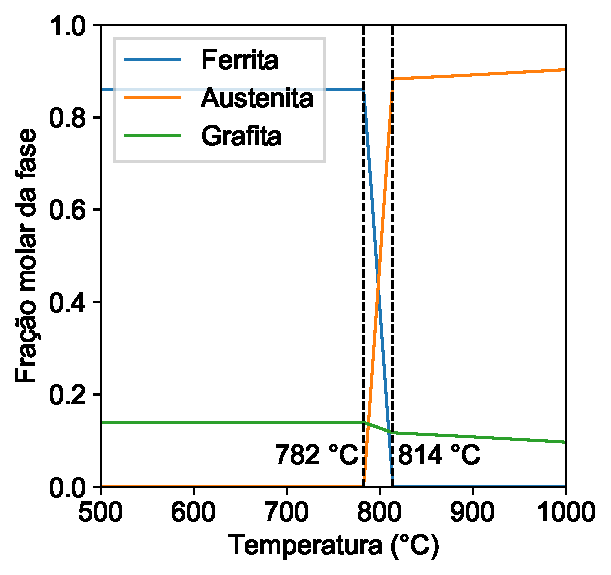
\includegraphics[width=7.5cm]{img/thermo-calc/NPvsT.png}}
	\quad
	\subfloat[]{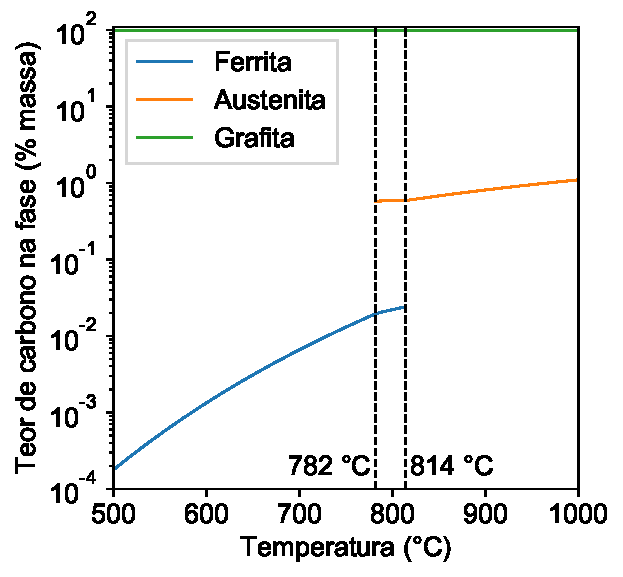
\includegraphics[width=7.5cm]{img/thermo-calc/CvsT.png}}
	\caption{Comportamento das frações de fases (a) e teor de carbono dissolvido nas fases em equilíbrio (b) em função da temperatura.}
	\label{fig:thermocalc}
\end{figure}

Os resultados obtidos no Thermo-Calc\textregistered{} também mostram como varia o teor de carbono dissolvido na austenita em função da temperatura. Nota-se que temperaturas maiores implicam em uma maior solubilidade do carbono na austenita, como já fora apontado na seção \ref{subsec:ADI}. A 814 °C, por exemplo, prevê-se que a austenita possuirá 0,59\%, enquanto que a 900 °C a solubilidade do carbono na austenita deverá ser de 0,81\%. Dessa forma, a martensita formada durante a têmpera após a austenitização em temperaturas mais elevadas tende a possuir morfologia de placas grossas e frágeis, enquanto temperaturas mais baixas devem gerar uma mistura de martensita em ripas e martensita em placas.

Para aferir as temperaturas correspondentes aos campos intercrítico e de austenitização plena previstas pelo Thermo-Calc\textregistered{} foi realizado um experimento de dilatometria para determinar as temperaturas críticas de transformação do material. Nas figuras \ref{fig:dilTempera}a e \ref{fig:dilTempera}b é mostrada a curva de dilatação para o ciclo de aquecimento do material e o resfriamento final. Em temperaturas inferiores a 737 °C (região A na figura \ref{fig:dilTempera}b) o material se dilata de forma aproximadamente linear, condizente com a expansão material em função do aumento da agitação térmica. A 737 °C, no entanto, é observada um súbito aumento da velocidade de expansão, observada em detalhe na figura \ref{fig:dilTempera}b, tendência que persiste até a temperatura de 783 °C (região B). Esta expansão é interpretada como a dissolução de carbonetos da microestrutura como recebida e formação de grafita, fase estável nesta temperatura. Entre 783 °C e 854 °C (região C) o material sofre outra transformação de fase, que leva a contração do material. Esta transformação, por sua vez, é associada à formação da fase compacta austenita, mais densa que os demais constituintes do ferro fundido. A partir de 854 °C (região D) a dilatação do material volta a ser aproximadamente linear, compatível com a expansão térmica da mistura de austenita e grafita.

\begin{figure}
	\subfloat[]{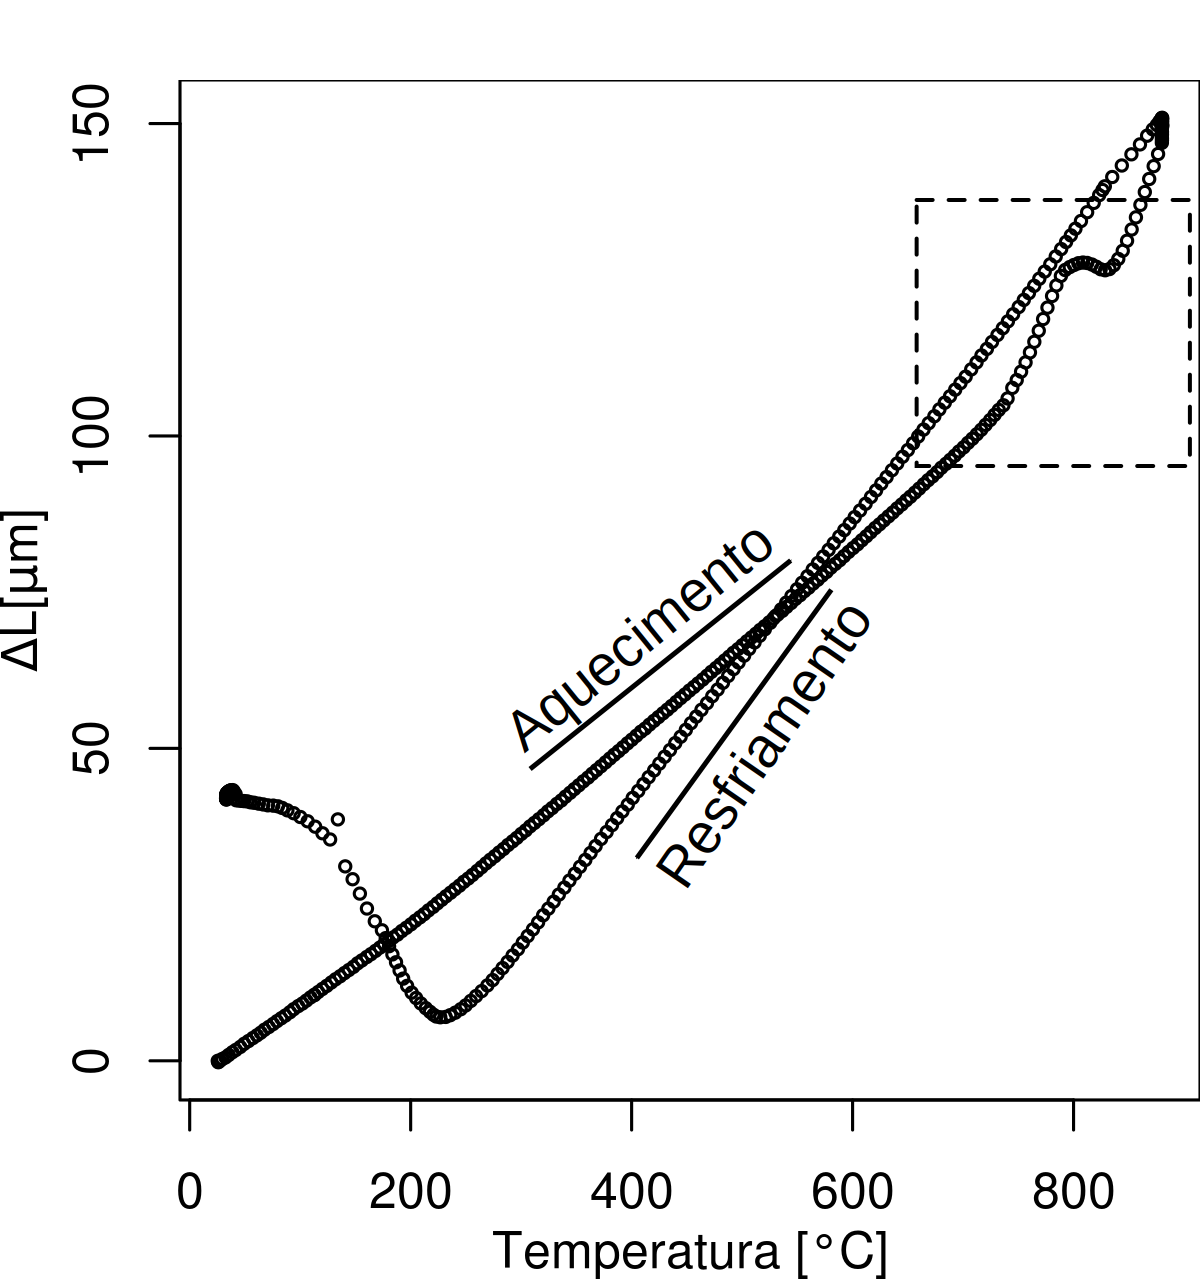
\includegraphics[height=7cm]{img/dilatometria/1_fofoTupy_10oCmin_2.png}}
	\quad
	\subfloat[]{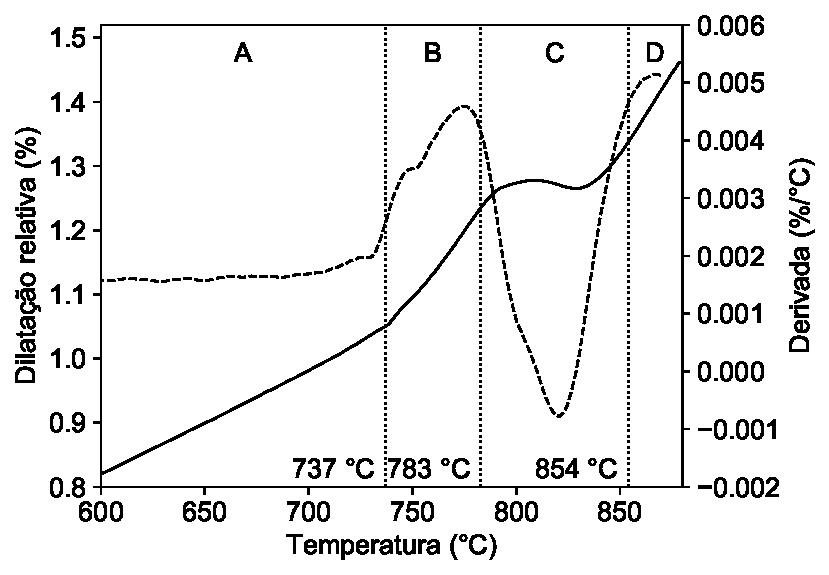
\includegraphics[height=7cm]{img/dilatometria/1_fofoTupy_10oCmin.png}}
	\caption{Curva de dilatação ($\Delta L$) em função da temperatura para o ferro fundido aquecido a 10 °C/min até a temperatura de 880 °C. (a) Curva completa. (b) Detalhe da curva (a) indicado pelo retângulo tracejado. A linha sólida corresponde à derivada numérica ($dL/dT$) da curva de dilatação em função da temperatura.}
	\label{fig:dilTempera}
\end{figure}

Quando comparada com os resultados da simulação termodinâmica, a interpretação da curva de dilatação mostra uma relação coerente entre a temperatura inferior do campo intecrítico (782 °C pelo Thermo-Calc\textregistered{} e 783 °C pela dilatometria), mas mostra uma discrepância entre as temperaturas de austenitização plena obtidas pelos dois métodos (814 °C pelo Thermo-Calc\textregistered{} e 854 °C pela dilatometria). Essa diferença pode ser justificada pela microsegregação do ferro fundido, que produz regiões com menor concentração de elementos gamagênicos, elevando localmente a temperatura de austenitização plena. Outra possibilidade é a própria inabilidade do banco de dados TCFE prever acuradamente o equilíbrio termodinâmico em sistemas complexos, uma vez que o software realiza extrapolações de informações termodinâmicas para prever os potenciais químicos dos elementos.

Para escolha da temperatura de austenitização, tomou-se como referência a menor temperatura em que se dá a austenitização plena do material, isto é, 854 °C. Uma menor temperatura de austenitização leva a uma austenita com menos carbono, implicando em uma martensita de caráter menos frágil do que a obtida em temperaturas mais elevadas de austenitização. Por outro lado, temperaturas elevadas beneficiam a homogeneização da segregação presente no material. Dessa forma, procurou-se adotar uma temperatura intermediária, que gerasse uma martensita de aspecto menos frágil, ao mesmo tempo que parte da heterogeneidade decorrente da segregação pudesse ser eliminada.

Dado o exposto, foi escolhida a temperatura de austenitização de 880 °C para os experimentos subsequentes. Nesta temperatura, o cálculo termodinâmico no software Thermo-Calc\textregistered{} prevê a composição química na austenita segundo a tabela \ref{tab:CQaust}.

\begin{table}
	\caption{Composição química da austenita determinada por cálculo termodinâmico no software Thermo-Calc\textregistered{}.}
	\begin{tabular}{c c c c c}
	\thickhline
	\textbf{Elemento} & C & Si & Mn & Cu\\
	\hline
	\textbf{Composição (\% em massa)} & 0,76 & 2.54 & 0,21 & 0,39\\
	\thickhline
	\end{tabular}
	\label{tab:CQaust}
\end{table}

\section{Dilatometria}

\subsection{Determina\c{c}\~{a}o da temperatura Ms}

A figura \ref{fig:dilMartensita}a mostra a curva de dilatação completa do ensaio de dilatometria para determinação da temperatura Ms. A expansão observada durante o resfriamento em torno de 230 °C corresponde à temperatura de início da transformação martensítica (Ms). Essa conclusão somente é possível de ser tomada caso a taxa de resfriamento de --50 °C/s aplicada à amostra tenha sido suficiente para garantir que a decomposição difusional da austenita tenha sido evitada. Análise metalográfica posterior (seção \ref{sec:micros}) confirma essa observação.

\begin{figure}
	\subfloat[]{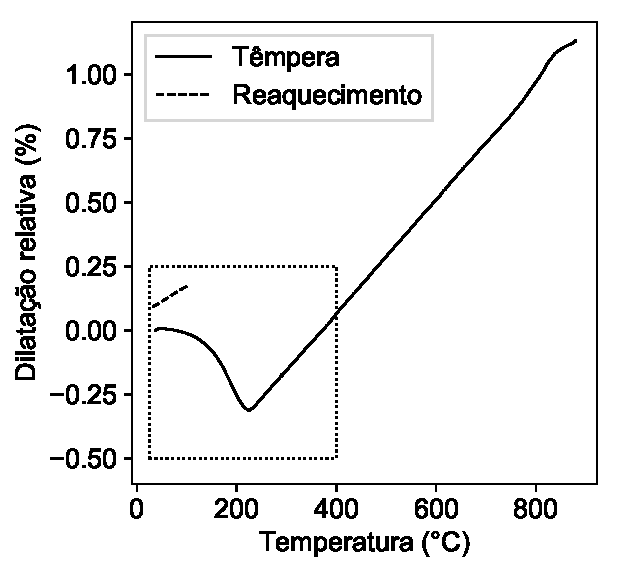
\includegraphics[height=9cm]{img/dilatometria/dil_martensita.png}}
	\vspace{0pt}
	\subfloat[]{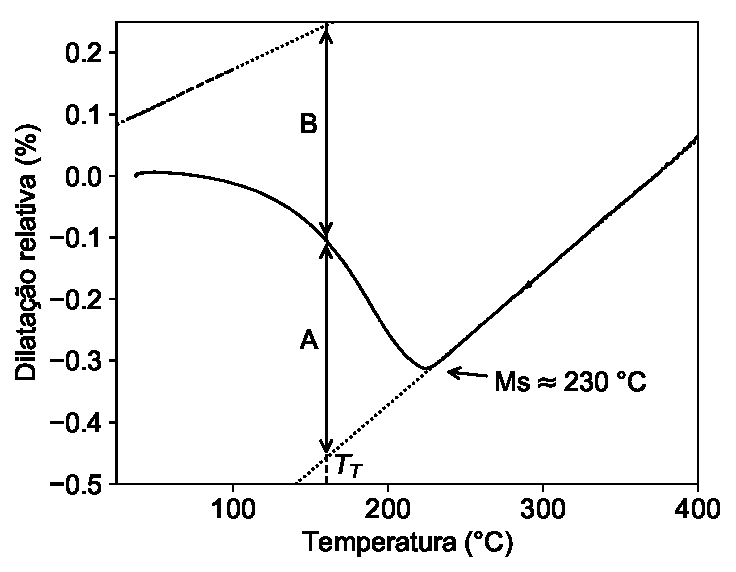
\includegraphics[height=9cm]{img/dilatometria/dil_martensita_close.png}}
	\caption{Curva de dilatação obtida durante o ciclo de austenitização e têmpera. (a) Curva completa. (b) Detalhe da expansão linear decorrente da transformação martensítica.}
	\label{fig:dilMartensita}
\end{figure}

Na figura \ref{fig:dilMartensita}b a expansão associada à reação martensítica é mostrada em detalhe. Em temperaturas superiores à Ms, a matriz do material é completamente austenítica. A dilatação da amostra nestas temperaturas é aproximadamente linear e é atribuída à agitação térmica. Em temperaturas inferiores à Ms a formação da martensita é acompanhada de uma forte expansão que cessa em uma temperatura de término da transformação martensítica (Mf) em que toda a austenita é consumida; nesse caso, a temperatura Mf se encontra em torno de --50 °C.

A fração transformada de martensita a partir da austenita $f^{\alpha\text{\textquoteright}}$ foi calculada utilizando a regra das alavancas, expressa pela equação \ref{eq:levelRule} expressa a seguir:

\begin{equation}
	f^{\alpha\text{\textquoteright}} = 1 - f^\gamma = \frac{A}{A + B}
	\label{eq:levelRule}
\end{equation}
%
em que $f^\gamma$ é a fração não transformada de austenita.

A determinação das variáveis ``A'' e ``B'' são mostradas na construção da figura \ref{fig:dilMartensita}b. ``A'' consiste da expansão associada à transformação martensítica em relação ao comprimento do corpo de prova caso ele permanecesse austenítico na temperatura de têmpera $TT$. Esse comprimento é determinado pela extrapolação do trecho de expansão térmica linear da austenita para a temperatura $TT$. $A + B$ é a expansão teórica do corpo de prova caso a amostra se transformasse completamente em martensita na temperatura $TT$.

A fração não transformada de austenita em função da temperatura de têmpera calculada pelo método exposto é mostrada na figura \ref{fig:KMFoFo}. Os dados experimentais, representados pelos círculos abertos, foram ajustados pelo método dos mínimos quadrados pelo modelo proposto por Koistinen e Marburger (equação \ref{eq:KM}). Na equação obtida o parâmetro de ajuste $\beta$ e a temperatura Ms foram determinados em $-1,23 \times 10^{-2} \text{°C}^{-1}$ e 221,1 °C, respectivamente. Nota-se que a temperatura Ms determinada como parâmetro de ajuste da equação de Koistinen-Marbuger é ligeiramente inferior àquela que corresponde ao início da expansão do corpo de prova em função da formação de martensita. Isso se deve a uma inércia para desencadeamento dos \textit{bursts} de martensita na austenita. Também se percebe que o coeficiente $\beta$ se mostrou bastante próximo ao valor de $-1,1 \times 10^{-2} \text{°C}^{-1}$ obtido no trabalho original de Koistinen e Marburger\cite{Koistinen1959}.

\begin{figure}
	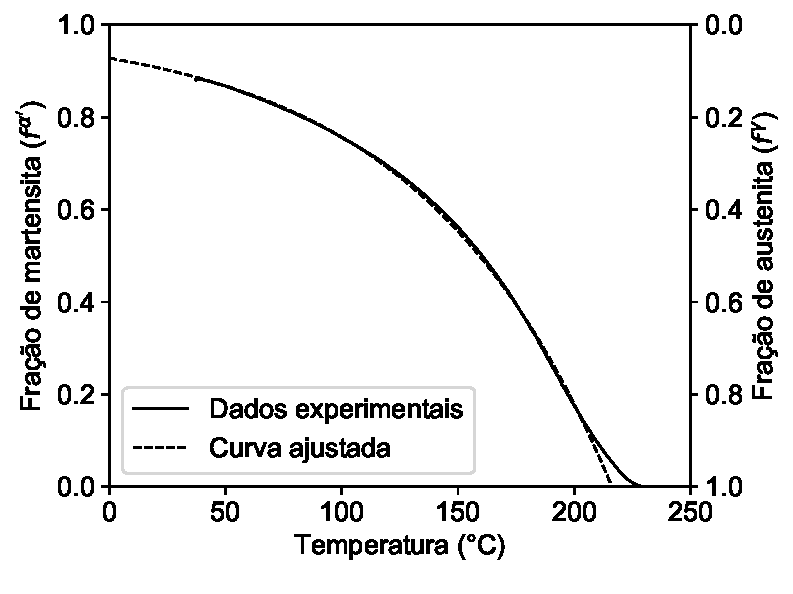
\includegraphics[height=12cm]{img/dilatometria/frac_martensita.png}
	\caption{Fração não transformada de austenita ($f^\gamma$) em função da temperatura de têmpera determinada pelos dados do experimento de dilatometria.}
	\label{fig:KMFoFo}
\end{figure}

Adicionalmente, a equação de Koistinen-Marburger não se ajusta bem aos valores experimentais para baixas temperaturas. Isso pode ser explicado pelo desvio da linearidade da expansão térmica para temperaturas muito baixas, tanto para a martensita, quanto para a austenita, como pontuado por \citaremsentenca{VanBohemen2013b}. A equação, no entanto, é perfeitamente válida para as temperaturas de têmpera utilizadas neste trabalho. Pela equação obtida, prevê-se que cerca de 9\% (em volume) de austenita é retida quando o material é temperado diretamente à temperatura ambiente (25 °C). A tabela \ref{tab:austRetida} mostra as quantidades de austenita não transformada que devem ser obtidas após a etapa de têmpera do ciclo T\&P programadas nos experimentos deste trabalho.

\begin{table}
	\caption{Porcentagem (em volume) de austenita não transformada obtida para diferentes temperaturas de têmpera.}
	\begin{tabular}{c c}
	\thickhline
	Temperatura de têmpera (TT) [°C] & \% em volume de austenita\\
	\hline
	25 &  9,0\\
	140 & 36,9\\ 
	170 & 53,3\\
	200 & 77,1\\
	\thickhline
	\end{tabular}
	\label{tab:austRetida}
\end{table}

\subsection{Resposta dilatom\'{e}trica durante ciclos t\'{e}rmicos T\&P}

As curvas representativas da dilatação e temperatura de um experimento de T\&P são mostradas na figura \ref{fig:TP170-300}a. Nesta condição, após a austenitização a 880 °C a amostra de dilatometria foi resfriada até a temperatura de 170 °C, na qual foi mantida por 60 segundos, sendo em seguida reaquecida até 300 °C e mantida por 15 minutos durante a etapa de partição. O final da etapa de resfriamento da têmpera é mostrado em detalhe na figura \ref{fig:TP170-300}b. Percebe-se que imediatamente após o início da etapa de têmpera a amostra sofre uma significativa expansão volumétrica, decorrente da transformação martensítica. Paralelamente, ocorre uma rápida elevação da temperatura, seguida de sua gradativa diminuição até o estabelecimento da temperatura de têmpera programada (i.e., 170 °C). Essa observação foi feita em todas as amostras submetidas ao ciclo T\&P. Isto acontece porque, devido ao resfriamento rápido, há a formação de um gradiente térmico na amostra que provoca uma diferença entre as temperaturas do núcleo e da superfície. Quando o fluxo de gás He --- utilizando no resfriamento forçado --- para, a temperatura da amostra tende a se homogeneizar, de modo que a superfície é reaquecida com o calor proveniente do centro, acarretando no aumento da temperatura medida pelo termopar. Além disso, a reação martensítica libera um calor latente de transformação, também colaborando para a elevação da temperatura.

\begin{figure}
	\subfloat[]{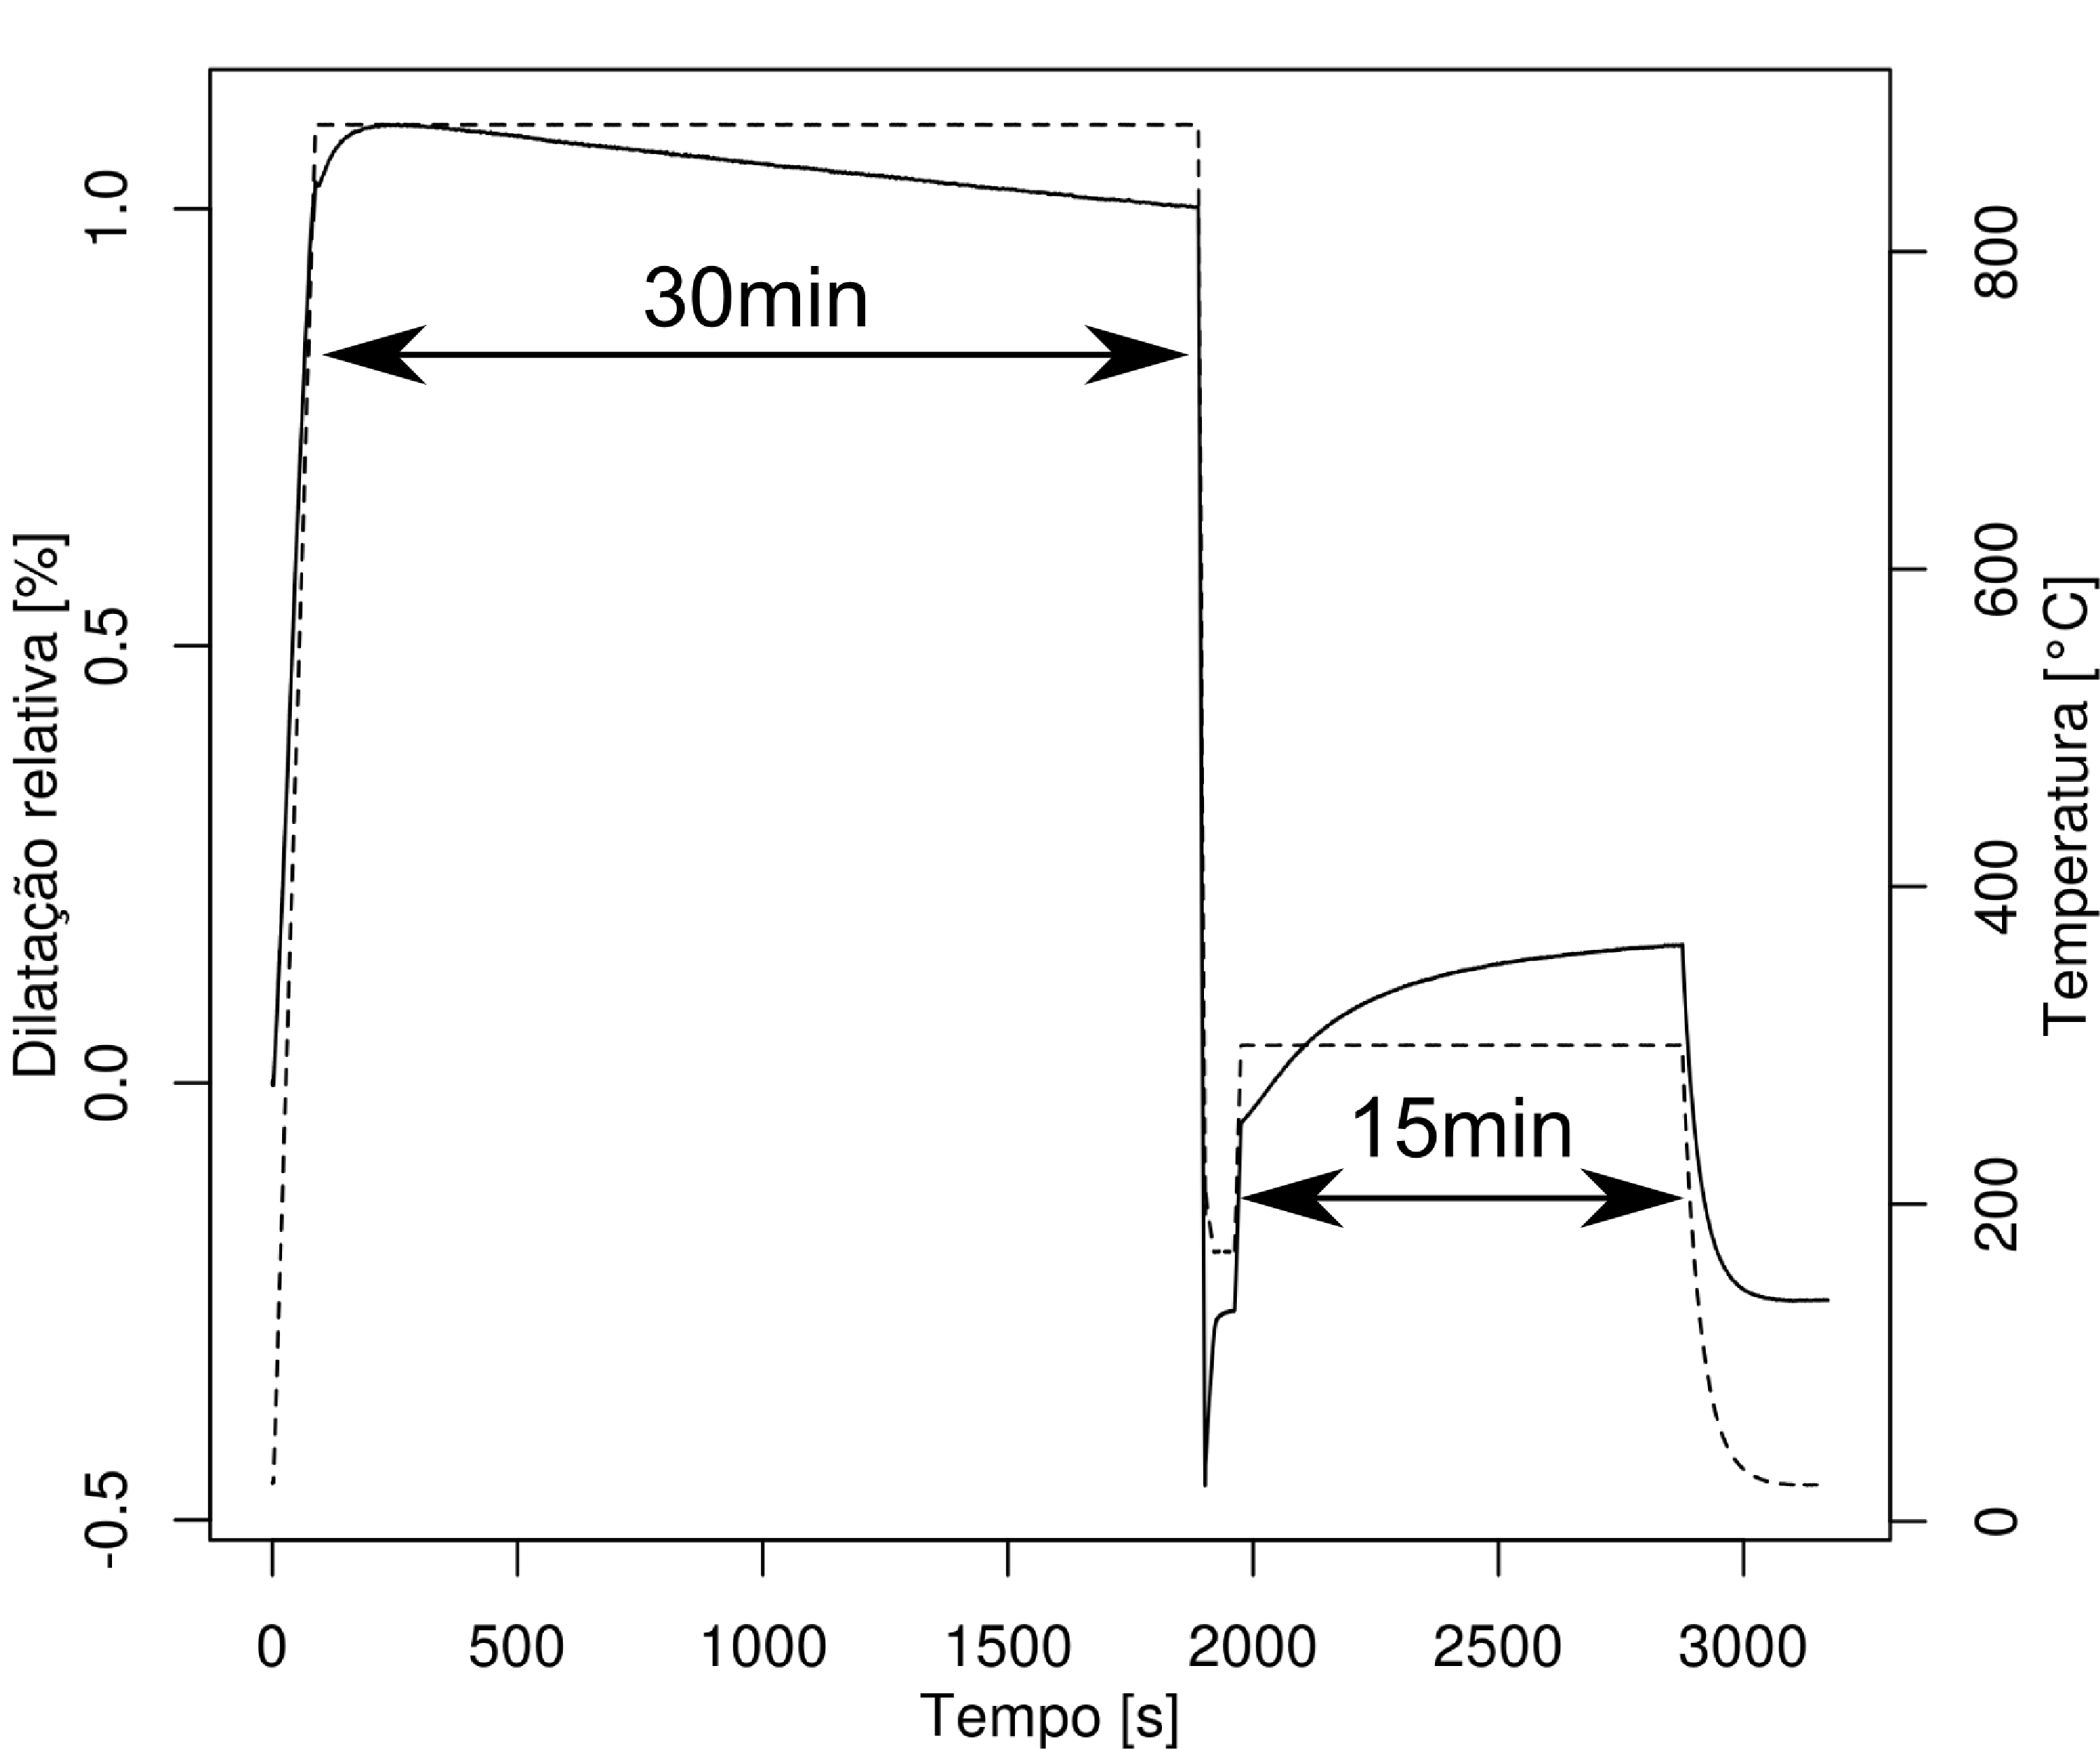
\includegraphics[height=9cm]{img/dilatometria/170-300.png}}
	\vspace{0pt}
	\subfloat[]{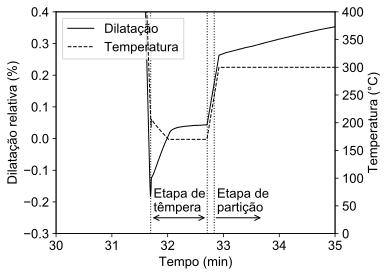
\includegraphics[height=9cm]{img/dilatometria/170-300_close.png}}
	\caption{Curvas de dilatação e temperatura em função do tempo para a amostra temperada a 170 °C e particionada a 300 °C por 15 minutos. (a) Curvas completas. (b) Detalhe do trecho final do resfriamento e do início da etapa de partição.}
	\label{fig:TP170-300}
\end{figure}

As figuras \ref{fig:PT200} a \ref{fig:PT450} mostram as curvas de dilatação durante a etapa isotérmica de partição em função do tempo (figuras com índice ``a'') e as curvas de dilatação em função da temperatura nas etapas adjacentes à etapa de partição (figuras com índice ``b''). Cada figura foi agrupada de acordo com uma temperatura de partição.

\begin{figure}
	\subfloat[]{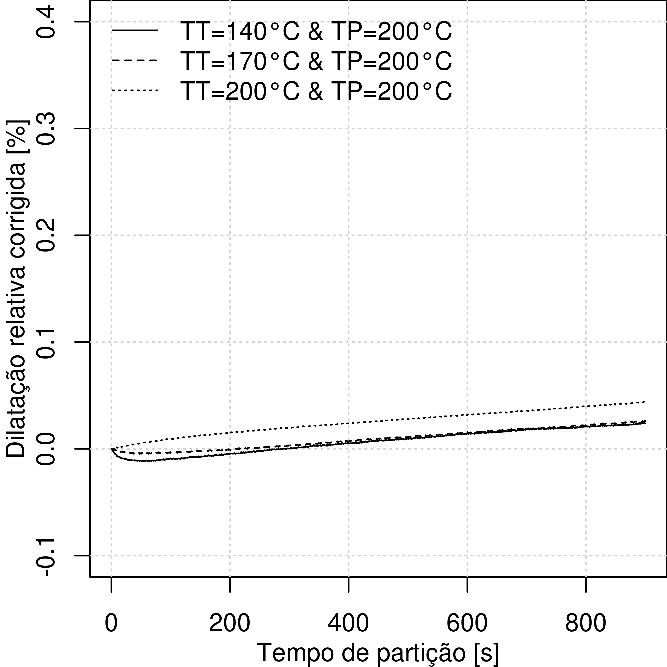
\includegraphics[width=7.5cm]{img/dilatometria/dilxtime_PT200.png}}
	\quad
	\subfloat[]{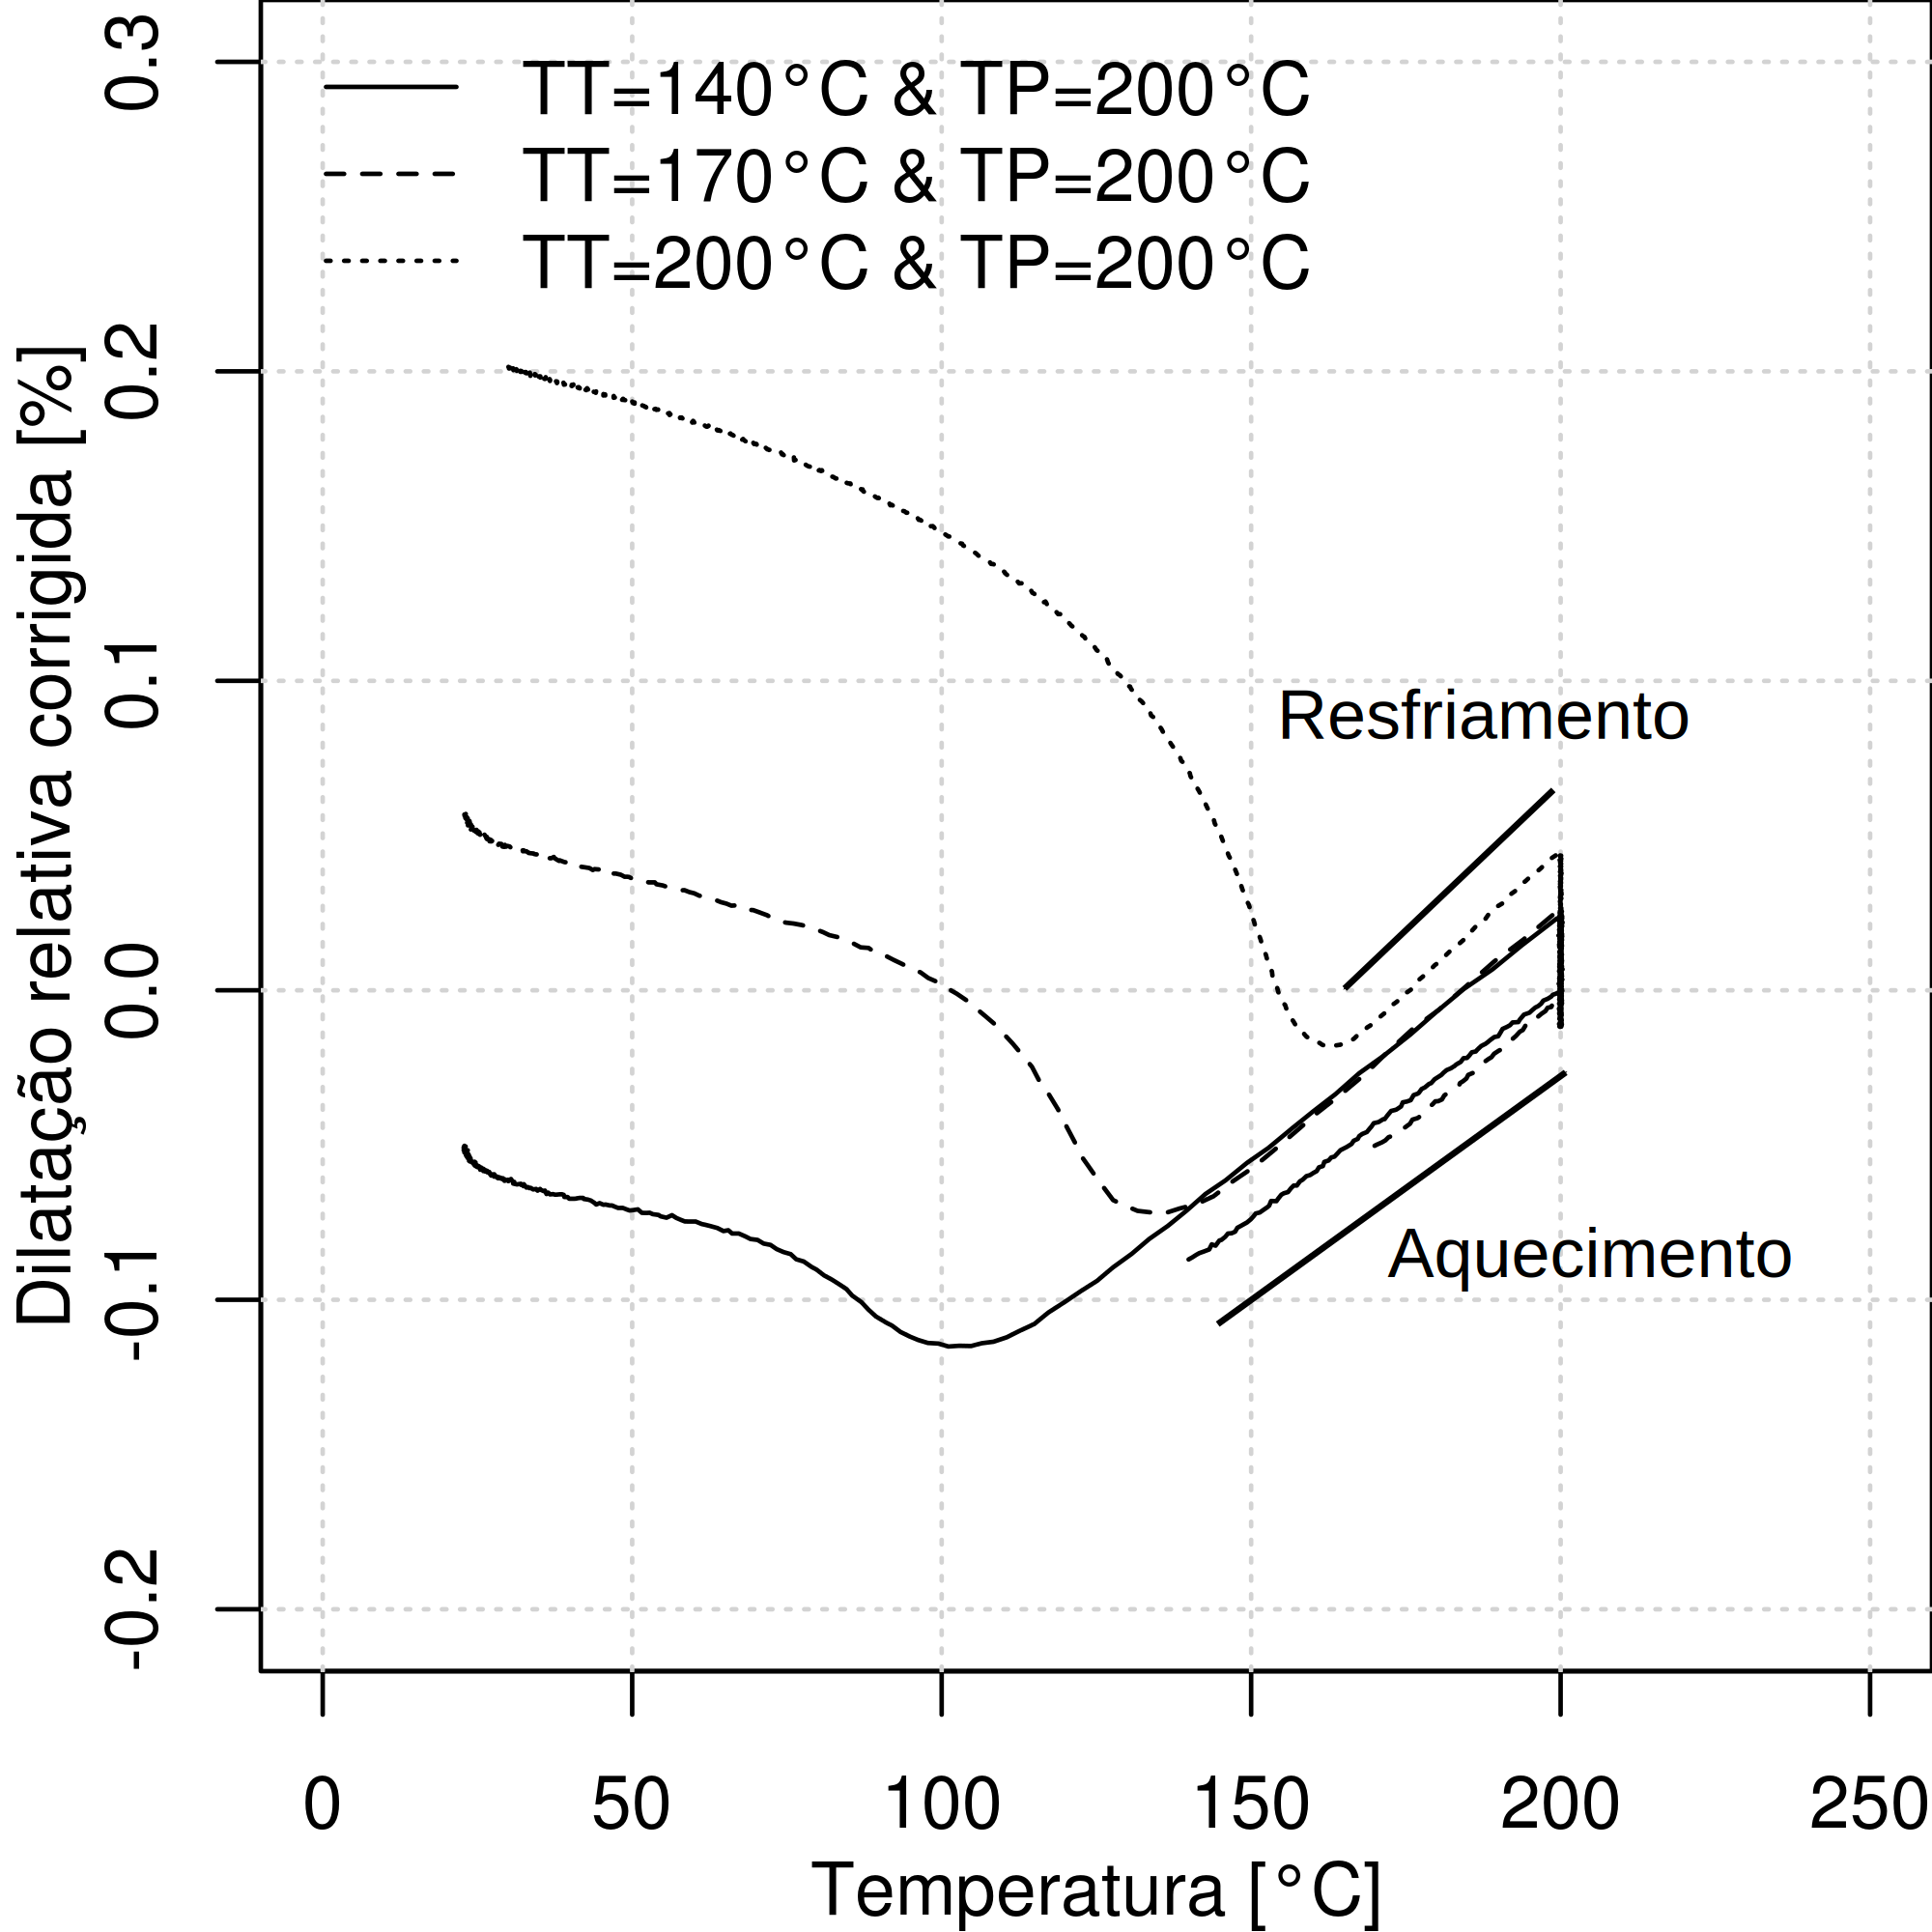
\includegraphics[width=7.5cm]{img/dilatometria/dilxT_PT200.png}}
	\caption{Curvas de dilatação das amostradas particionadas a 200 °C. (a) Dilatação relativa durante a etapa de partição em função do tempo. (b) Dilatação relativa em função da temperatura.}
	\label{fig:PT200}
\end{figure}

\begin{figure}
	\subfloat[]{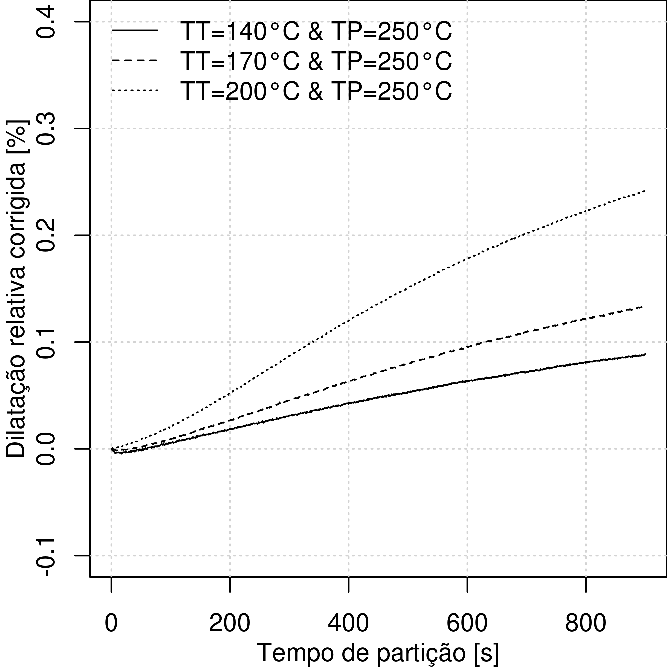
\includegraphics[width=7.5cm]{img/dilatometria/dilxtime_PT250.png}}
	\quad
	\subfloat[]{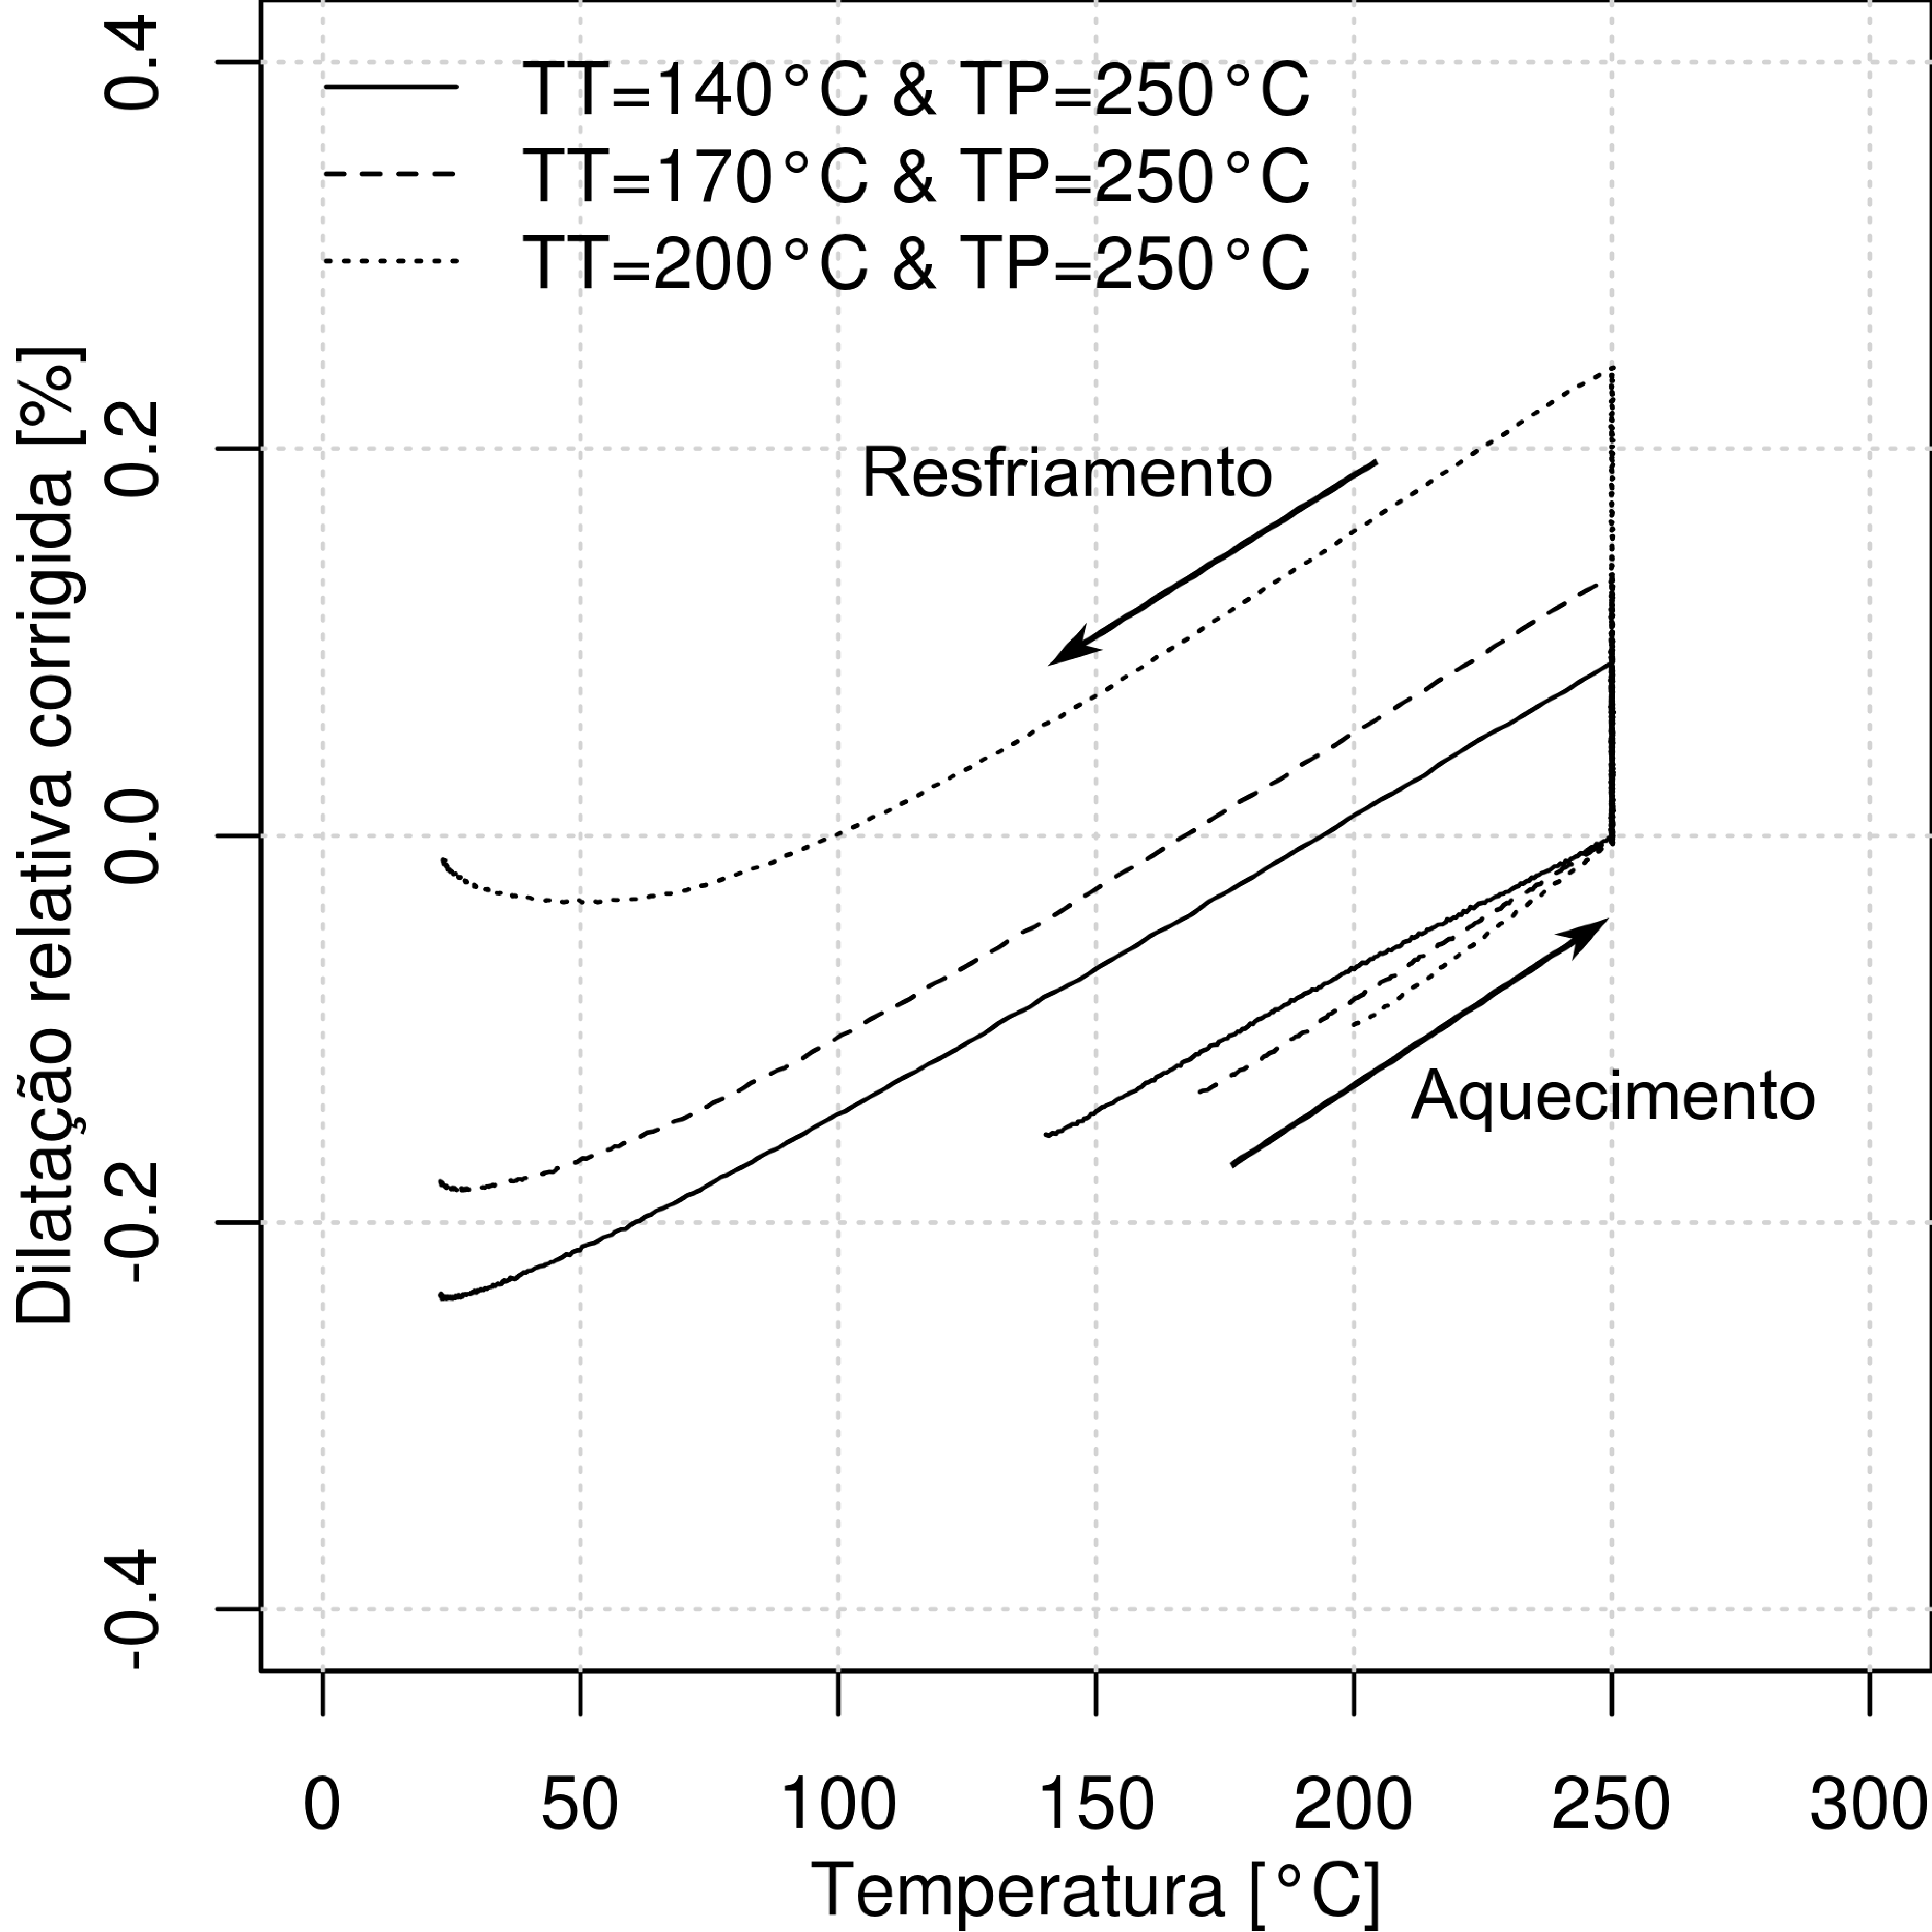
\includegraphics[width=7.5cm]{img/dilatometria/dilxT_PT250.png}}
	\caption{Curvas de dilatação das amostradas particionadas a 250 °C. (a) Dilatação relativa durante a etapa de partição em função do tempo. (b) Dilatação relativa em função da temperatura.}
	\label{fig:PT250}
\end{figure}

\begin{figure}
	\subfloat[]{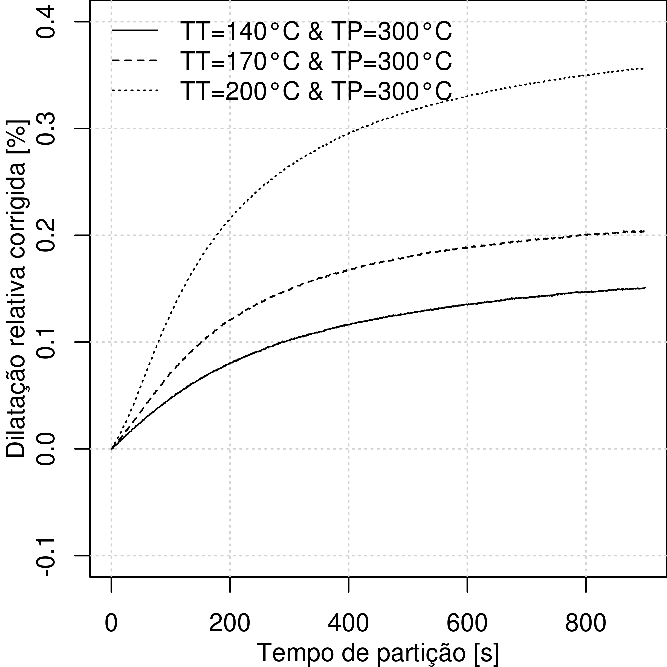
\includegraphics[width=7.5cm]{img/dilatometria/dilxtime_PT300.png}}
	\quad
	\subfloat[]{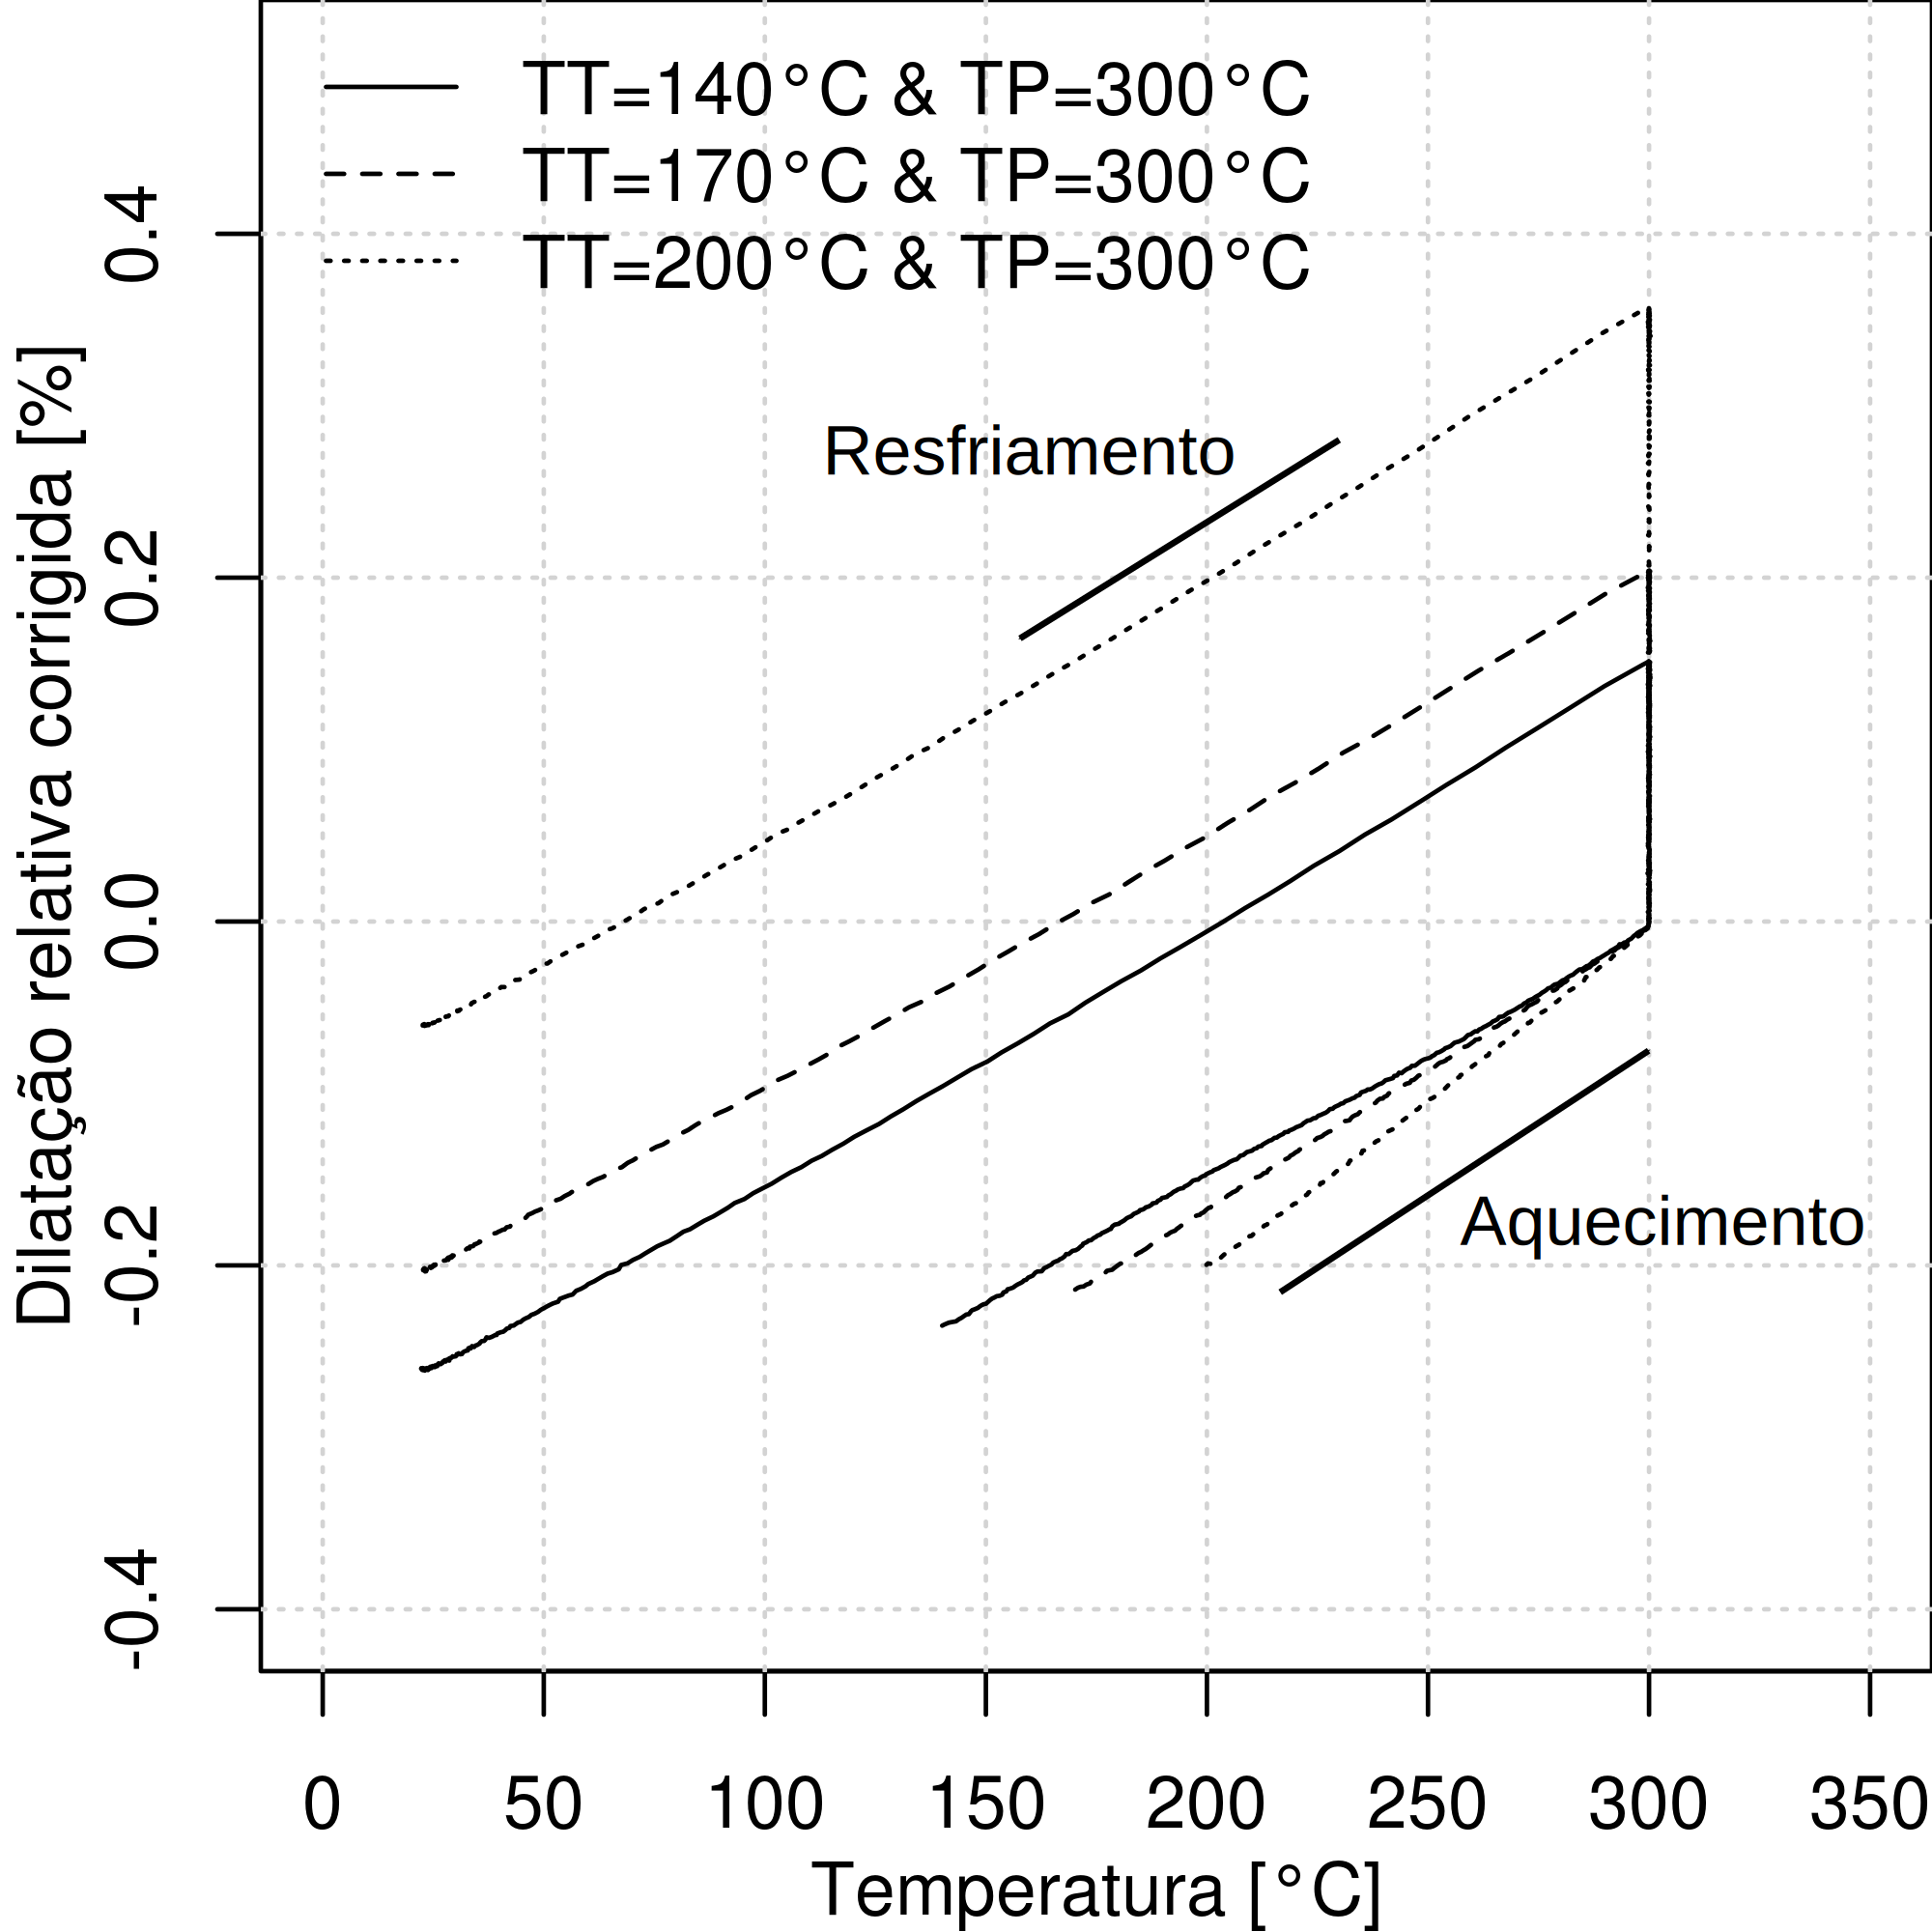
\includegraphics[width=7.5cm]{img/dilatometria/dilxT_PT300.png}}
	\caption{Curvas de dilatação das amostradas particionadas a 300 °C. (a) Dilatação relativa durante a etapa de partição em função do tempo. (b) Dilatação relativa em função da temperatura.}
	\label{fig:PT300}
\end{figure}

\begin{figure}
	\subfloat[]{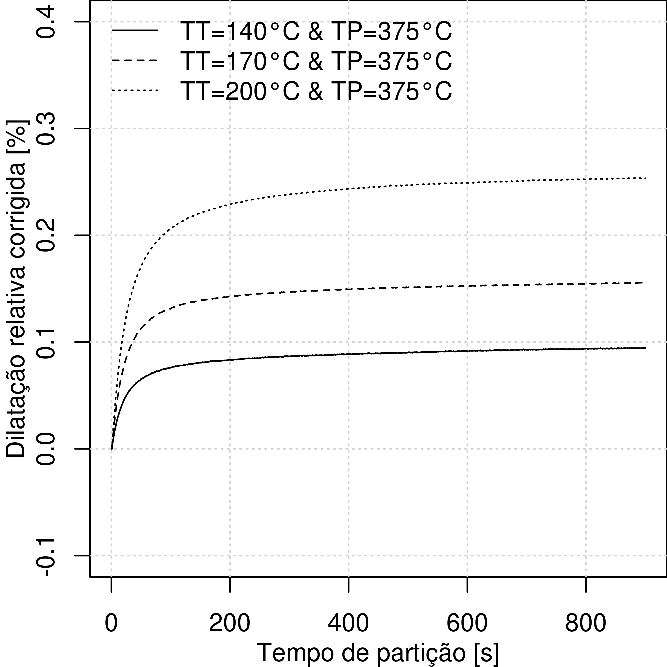
\includegraphics[width=7.5cm]{img/dilatometria/dilxtime_PT375.png}}
	\quad
	\subfloat[]{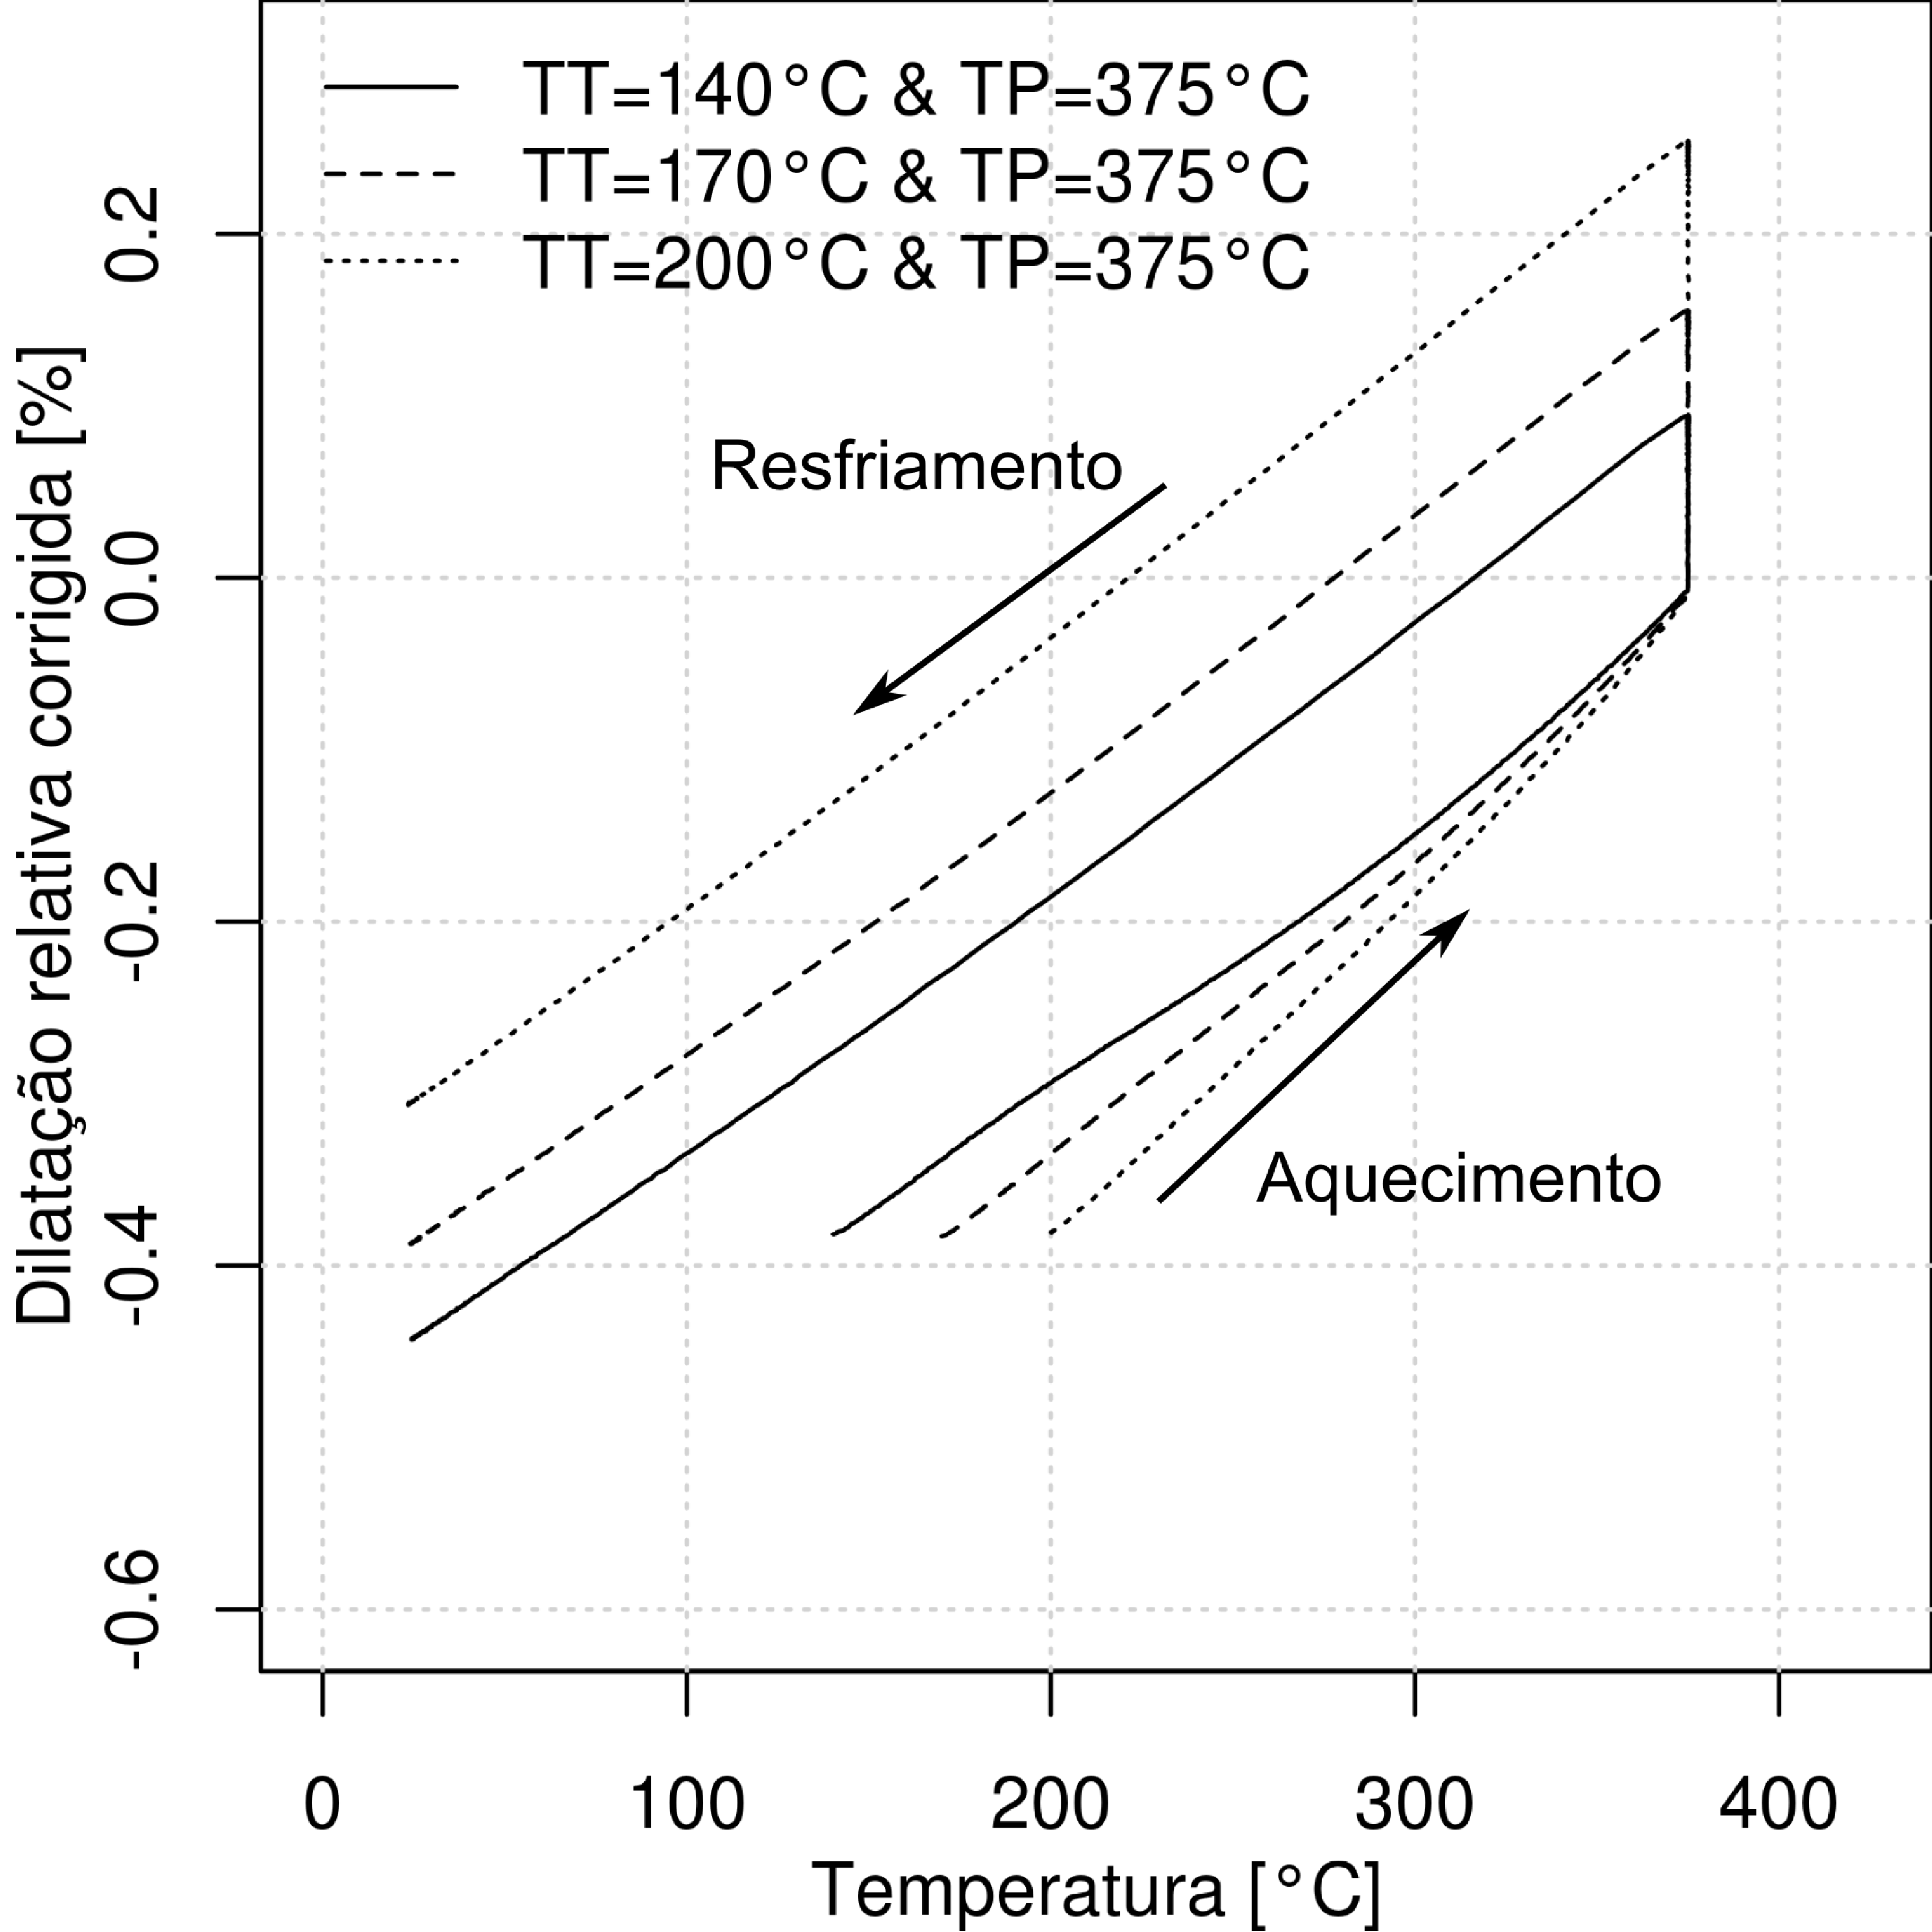
\includegraphics[width=7.5cm]{img/dilatometria/dilxT_PT375.png}}
	\caption{Curvas de dilatação das amostradas particionadas a 375 °C. (a) Dilatação relativa durante a etapa de partição em função do tempo. (b) Dilatação relativa em função da temperatura.}
	\label{fig:PT375}
\end{figure}

\begin{figure}
	\subfloat[]{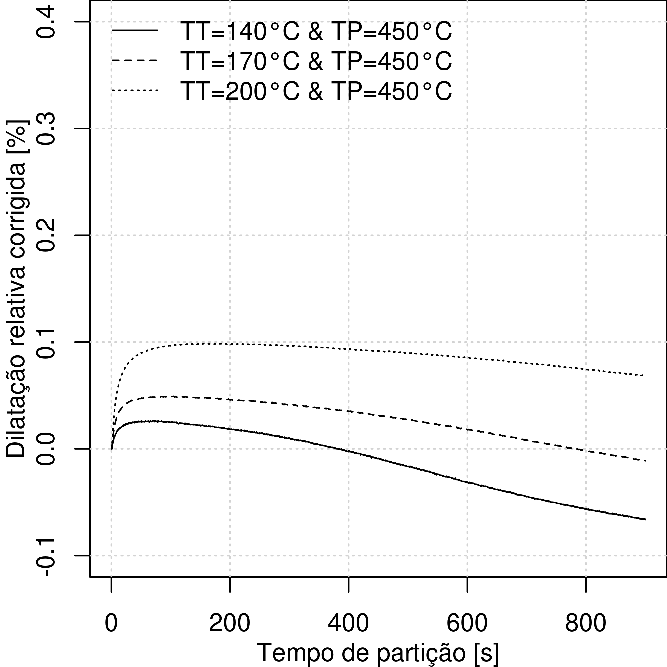
\includegraphics[width=7.5cm]{img/dilatometria/dilxtime_PT450.png}}
	\quad
	\subfloat[]{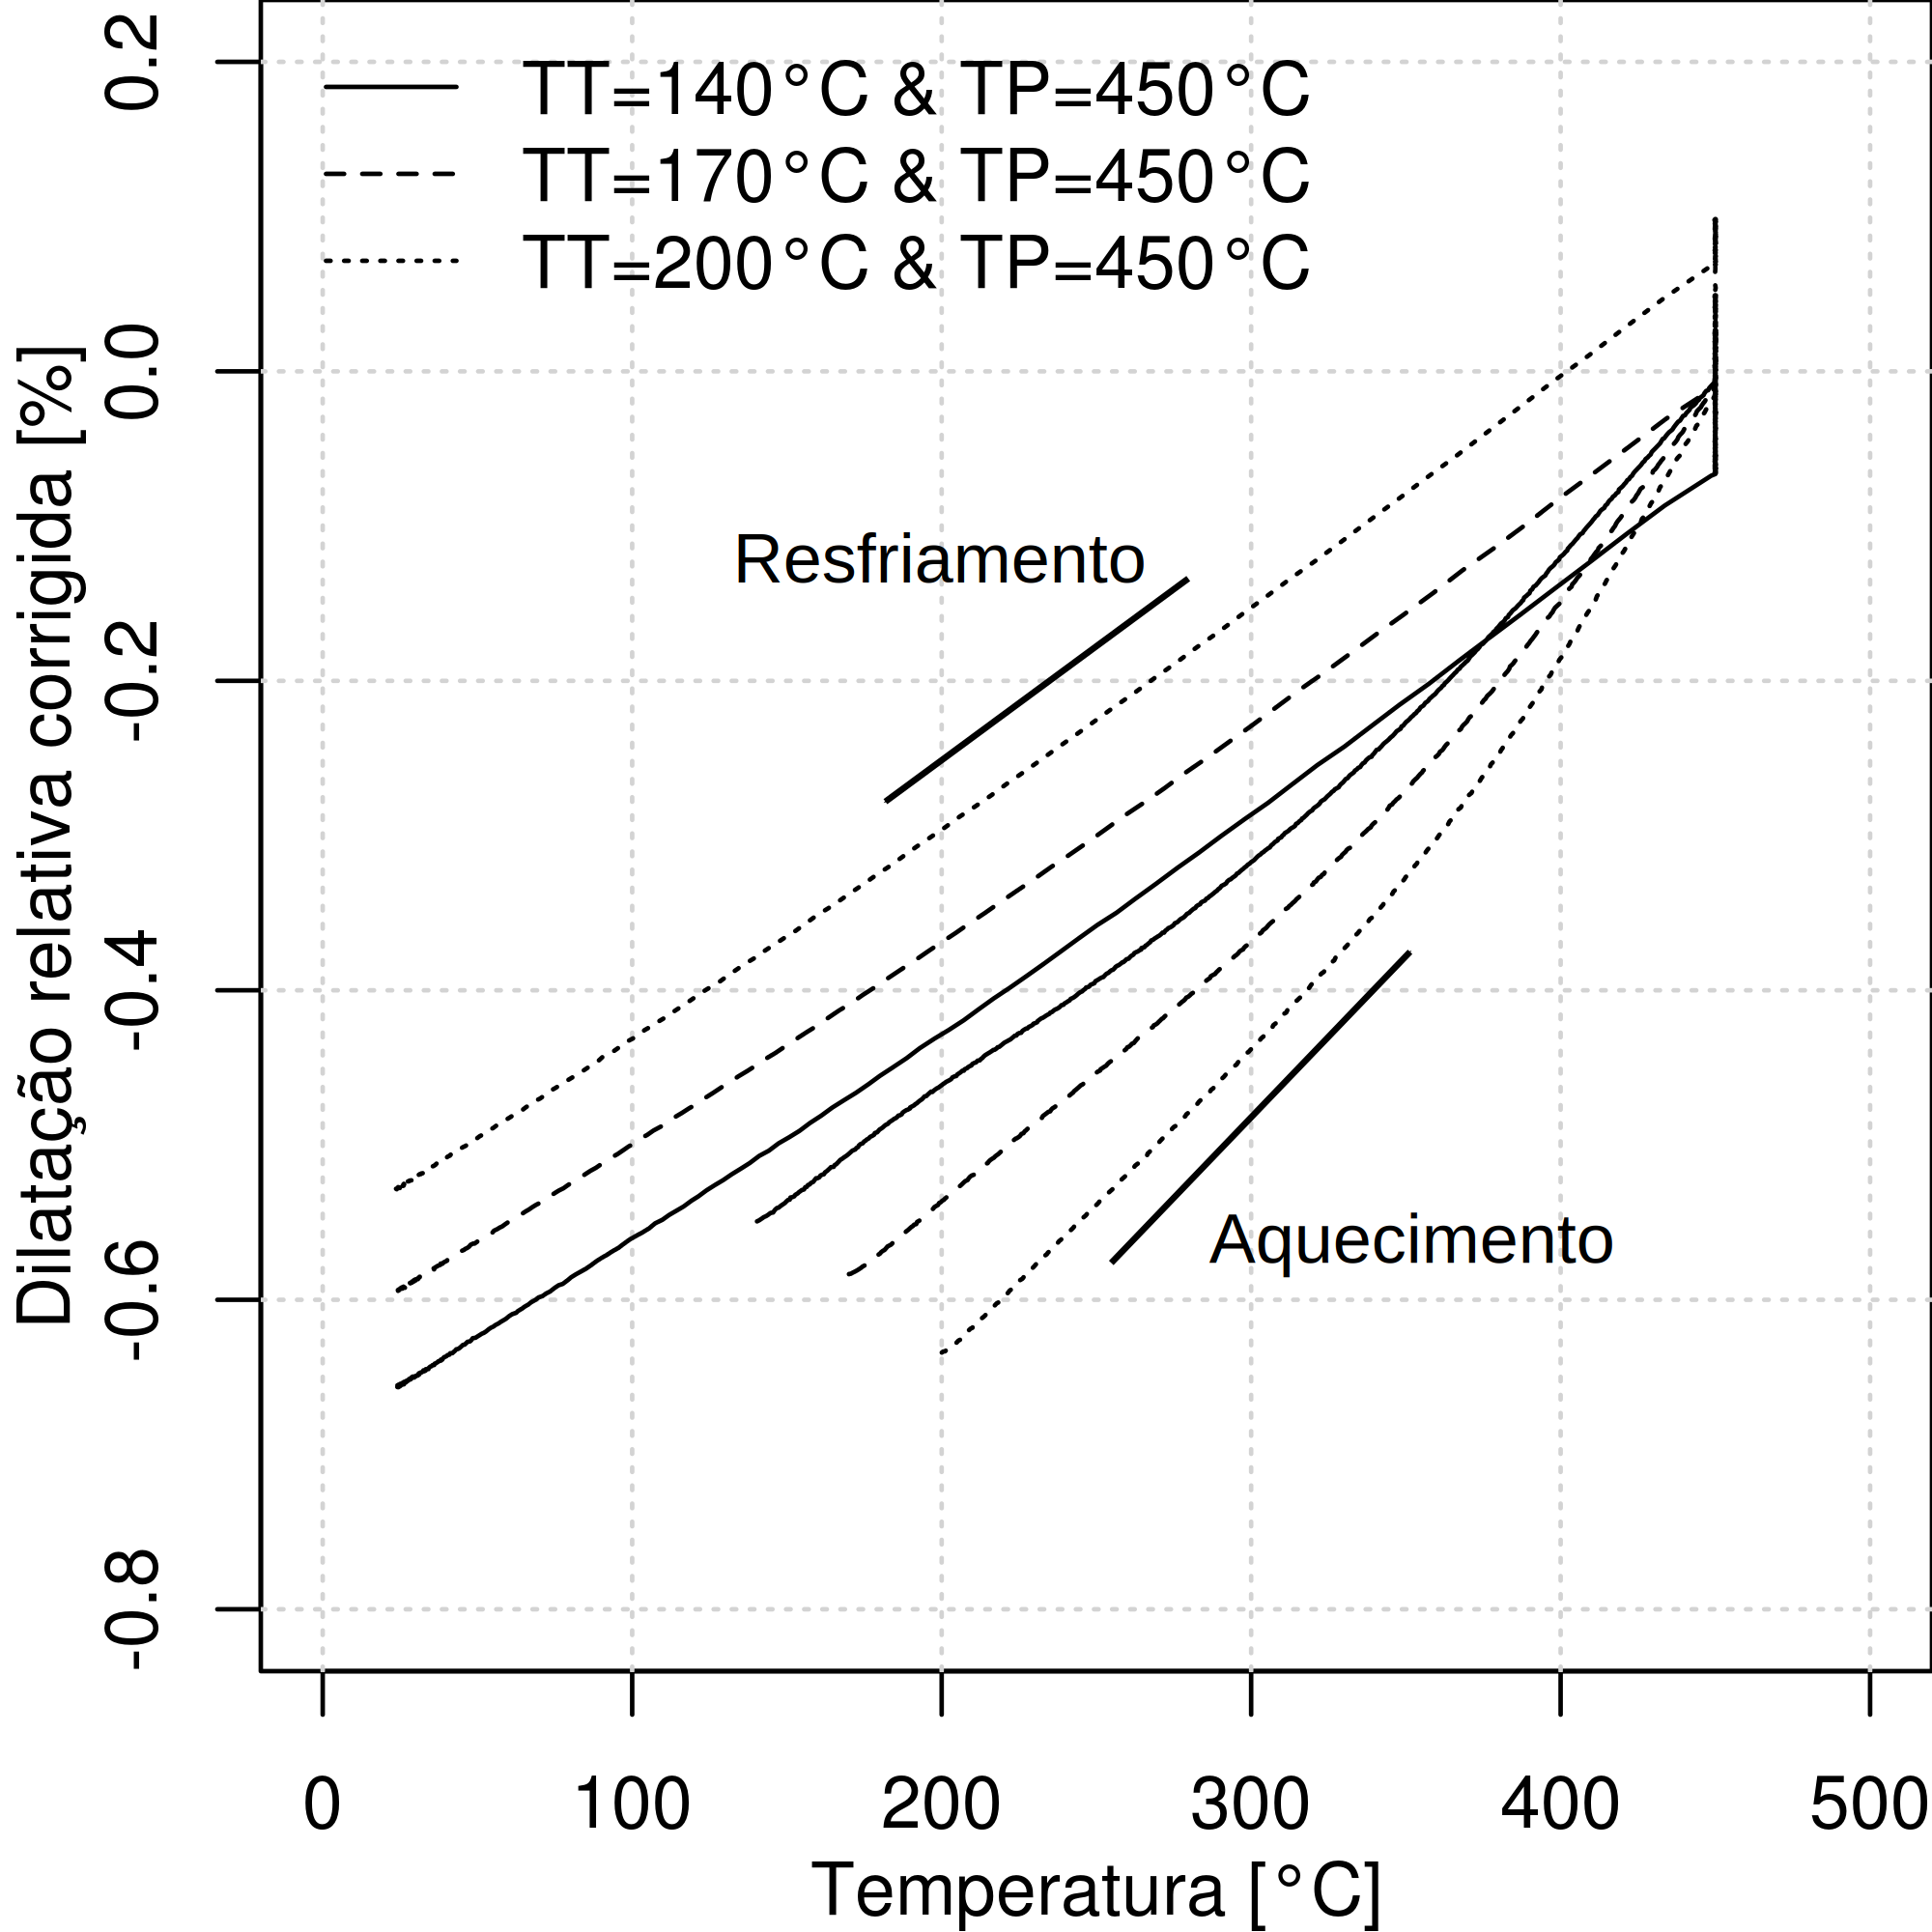
\includegraphics[width=7.5cm]{img/dilatometria/dilxT_PT450.png}}
	\caption{Curvas de dilatação das amostradas particionadas a 450 °C. (a) Dilatação relativa durante a etapa de partição em função do tempo. (b) Dilatação relativa em função da temperatura.}
	\label{fig:PT450}
\end{figure}

Mudanças no comprimento das amostras são previstas pela redistribuição de carbono da martensita para a austenita. Como pontuado na seção \ref{subsubsec:ERC}, a redistribuição de carbono segundo o modelo de equilíbrio restringido de carbono (ERC) leva a um ligeiro aumento da fração molar de austenita no material. Consequentemente, nesta situação a partição de carbono poderia vir acompanhada de uma pequena contração do material. Isto é observado apenas nas amostras particionadas a 200 °C temperadas a 140 e 170 °C (figura \ref{fig:PT200}a). Nestas amostras a contração inicial do material é procedida por uma pequena dilatação. Em todas as outras amostras há significativa expansão volumétrica durante os primeiros instantes de partição. Nas amostras particionadas a 450 °C (figura \ref{fig:PT450}) o período de expansão volumétrica é curto (cerca de 60 segundos) e no intervalo de tempo subsequente ocorre a contração das amostras.

As mudanças no comprimento das amostras particionadas em temperaturas maiores que 200 °C não podem ser explicadas pela partição de carbono segundo o modelo ERC e, portanto, são indicativos da ocorrência de reações competitivas que consomem a austenita na etapa de partição. Uma vez que as temperaturas de partição utilizadas neste trabalho são semelhantes às utilizadas no tratamento de austêmpera nos ADIs, a suspeita óbvia é que as ilhas de austenita não-transformadas são gradativamente consumidas pela reação bainítica (formação de ausferrita) durante a partição. Como nos ADIs, a reação bainítica também deve funcionar como mecanismo de enriquecimento em carbono da austenita, desde que a precipitação de carbonetos do segundo estágio da reação seja retardada.

Observa-se também uma tendência bastante clara de que temperaturas maiores têmpera levam a maiores expansões volumétricas durante a etapa de partição. Isso decorre das maiores quantidades de austenita não-transformada presentes para temperaturas maiores têmpera, disponível para decompor para o produto bainítico durante a etapa isotérmica de partição. Além disso, as amostras particionadas a 300 °C foram as que sofreram maior expansão (em torno de 0,35\% para a amostra temperada a 200 °C). Por outro lado, a contração observada durante a etapa de partição a 450 °C (figura \ref{fig:PT450}a) é tão maior quanto maior a temperatura de têmpera.

No que diz respeito ao aspecto cinético da transformação isotérmica, nota-se que as curvas de dilatação não apresentam uma etapa inicial lenta, tal qual é observada nas curvas cinéticas características previstas pelo modelo de Johnson-Mehl-Avrami-Kolmogorov (JMAK). Isso possivelmente decorre da formação de núcleos do produto bainítico durante o aquecimento desde a temperatura de têmpera até a temperatura de partição. Outra possível hipótese é que as placas de martensita formadas durante a têmpera exercem algum efeito catalizador na reação isotérmica, diminuindo a barreira de ativação para nucleação da nova fase. Hipótese semelhante foi elaborada por \citaremsentenca{Oka1988} para justificar a aceleração da reação bainítica (\textit{swing back}) em temperaturas próximas ao Ms em aços carbono.

Outra característica a ser notada é a ocorrência, durante o resfriamento final, da formação de martensita a partir da austenita que não foi suficientemente enriquecida em carbono após o término da etapa de partição. Pelas figuras \ref{fig:PT200}b e \ref{fig:PT250}b observa-se uma expansão associada à reação martensítica durante o resfriamento final nas amostras particionadas a 200 e 250 °C. Conclui-se que a austenita produzida nestas condições, de fato, não adquiriu estabilidade suficiente para ser completamente retida à temperatura ambiente. Por outro lado, nas demais amostras não foi observada expansão semelhante, ou seja, não é observada uma temperatura Ms durante o resfriamento final. Isto é associado a dois motivos: ou a austenita foi completamente estabilizada pela redistribuição de carbono durante a partição, ou a austenita foi completamente consumida pelas reações competitivas. A ocorrência de um ou outro fenômeno é discutida por meio dos resultados de difração de raios X (seção \ref{sec:DRXInSitu}).

A tabela \ref{tab:MsTP} sumariza as temperaturas Ms determinadas para cada condição estudada. Nas condições em que não houve suficiente estabilização da austenita a temperatura Ms obtida é tão maior quando menor a temperatura de têmpera. Menores temperatura de têmpera geram maiores quantidades de martensita. Nessa condição há ``mais carbono'' disponível para ser redistribuído da martensita para a austenita não transformada durante a partição. Consequentemente, a austenita particionada após a têmpera em temperaturas mais baixas acaba adquirindo um caráter mais estável do que a obtida quando a têmpera é feita em temperaturas maiores.

\begin{table}
	\caption{Temperaturas Ms determinadas para cada condição estudada após o processo T\&P.}
	\begin{tabular}{c c c ' c c c}
	\thickhline
	TT [°C] & TP [°C] & Ms [°C] & TT [°C] & TP [°C] & Ms [°C]\\
	\hline
	140 & 200 & 119 & 140 & 375 & < 25\\
	170 & 200 & 148 & 170 & 375 & < 25\\
	200 & 200 & 168 & 200 & 375 & < 25\\
	\hline
	140 & 250 & 35 & 140 & 450 & < 25\\
	170 & 250 & 77 & 170 & 450 & < 25\\
	200 & 250 & 109 & 200 & 450 & < 25\\
	\hline
	140 & 300 & < 25 &&&\\
	170 & 300 & < 25 &&&\\
	200 & 300 & < 25 &&&\\
	\thickhline
	\end{tabular}
	\label{tab:MsTP}
\end{table}

Assumindo que a diminuição da temperatura Ms é consequente do enriquecimento em carbono da austenita, é possível estimar o acréscimo $\Delta \%w_C^\gamma$ em carbono da austenita durante a etapa de partição pela equação de Andrews (equação \ref{eq:Andrews}). Nesta equação, o coeficiente de valor 423 que acompanha a variável $\%w_C^\gamma$ significa que o aumento de 1\% no teor de carbono da austenita provoca a diminuição de 423 °C na temperatura Ms desta fase. Com base nesse raciocínio, a tabela \ref{tab:wCgammaAndrews}, sumarizando os valores de $\Delta \%w_C^\gamma$ para as condições de tratamento térmico foi obtida.

\begin{table}
	\caption{Estimativa da variação no teor de carbono da austenita ($\Delta \%w_C^\gamma$) após o processo T\&P para cada condição de tratamento térmico.}
	\begin{tabular}{c c c ' c c c}
	\thickhline
	TT [°C] & TP [°C] & $\Delta \%w_C^\gamma$ & TT [°C] & TP & $\Delta \%w_C^\gamma$\\
	\hline
	140 & 200 & 0,26 & 140 & 375 & > 0,48\\
	170 & 200 & 0,19 & 170 & 375 & > 0,48\\
	200 & 200 & 0,15 & 200 & 375 & > 0,48\\
	\hline
	140 & 250 & 0,46 & 140 & 450 & > 0,48\\
	170 & 250 & 0,36 & 170 & 450 & > 0,48\\
	200 & 250 & 0,29 & 200 & 450 & > 0,48\\
	\hline
	140 & 300 & > 0,48 &&&\\
	170 & 300 & > 0,48 &&&\\
	200 & 300 & > 0,48 &&&\\
	\thickhline
	\end{tabular}
	\label{tab:wCgammaAndrews}
\end{table}

\subsection{Resposta dilatom\'{e}trica durante ciclos t\'{e}rmicos de aust\^{e}mpera}

Uma vez que foram observadas expansões volumétricas significativas durante a etapa de partição do processo T\&P e foi levantada a hipótese de que estas variações no comprimento estariam associadas a reações semelhantes às observadas durante a produção de ADIs, tratamentos isotérmicos de austêmpera foram realizados para se determinar o comportamento cinético da reação bainítica no ferro nodular estudado. A figura \ref{fig:IBT} ilustra este comportamento durante o patamar isotérmico de austêmpera.

\begin{figure}
	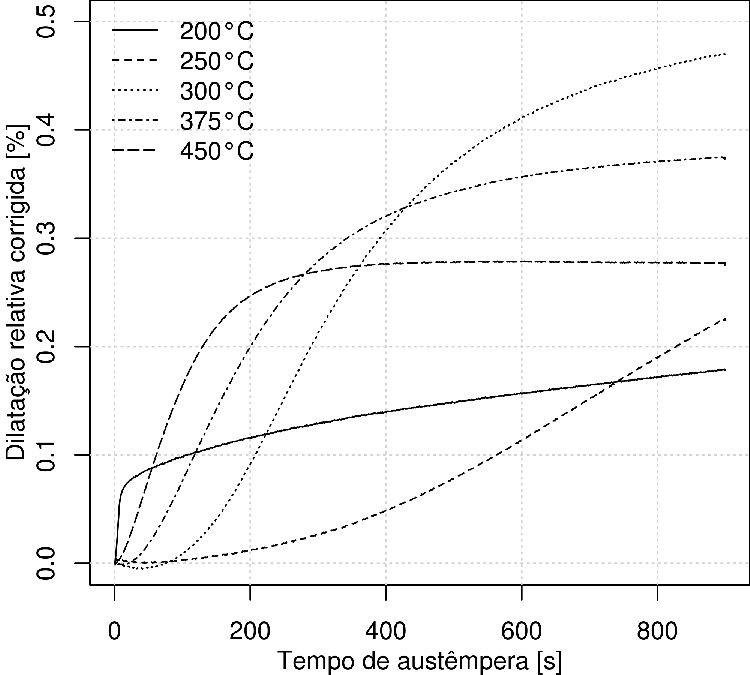
\includegraphics[height=12cm]{img/dilatometria/dilation_IBT.png}
	\caption{Curvas de dilatação das amostradas tratadas isotermicamente entre 200 e 450 °C.}
	\label{fig:IBT}
\end{figure}

Observa-se que em todas as condições estudadas há sensível expansão das amostras. Com exceção das amostras austemperadas a 200 °C, pode-se concluir em todas as condições as curvas dilatométricas apresentaram um formato sigmoidal característico, compatível com a descrição cinética prevista pela equação de JMAK. Isto é interpretado pela lenta cinética no começo da transformação, associada à etapa de nucleação da fase produto, procedida por uma rápida expansão, relacionada ao crescimento do produto bainítico.

Dentre as amostras tratadas entre 300 e 450 °C, menores temperaturas de tratamento isotérmico produziram maiores expansões volumétricas dos corpos de prova. Isto é justificado pela diferença entre os valores dos coeficientes de expansão térmica da austenita e da ferrita, maior para a primeira a fase. Como pode ser observado na figura \ref{fig:dilRel}, estas diferenças afetam a dilatação produzida pela formação da ferrita (fase cúbica de corpo centrado) a partir da austenita (fase cúbica de face centrada). A mesma justificativa pode ser utilizada para explicar os resultados obtidos nas amostras tratadas pelo processo T\&P.

\begin{figure}
	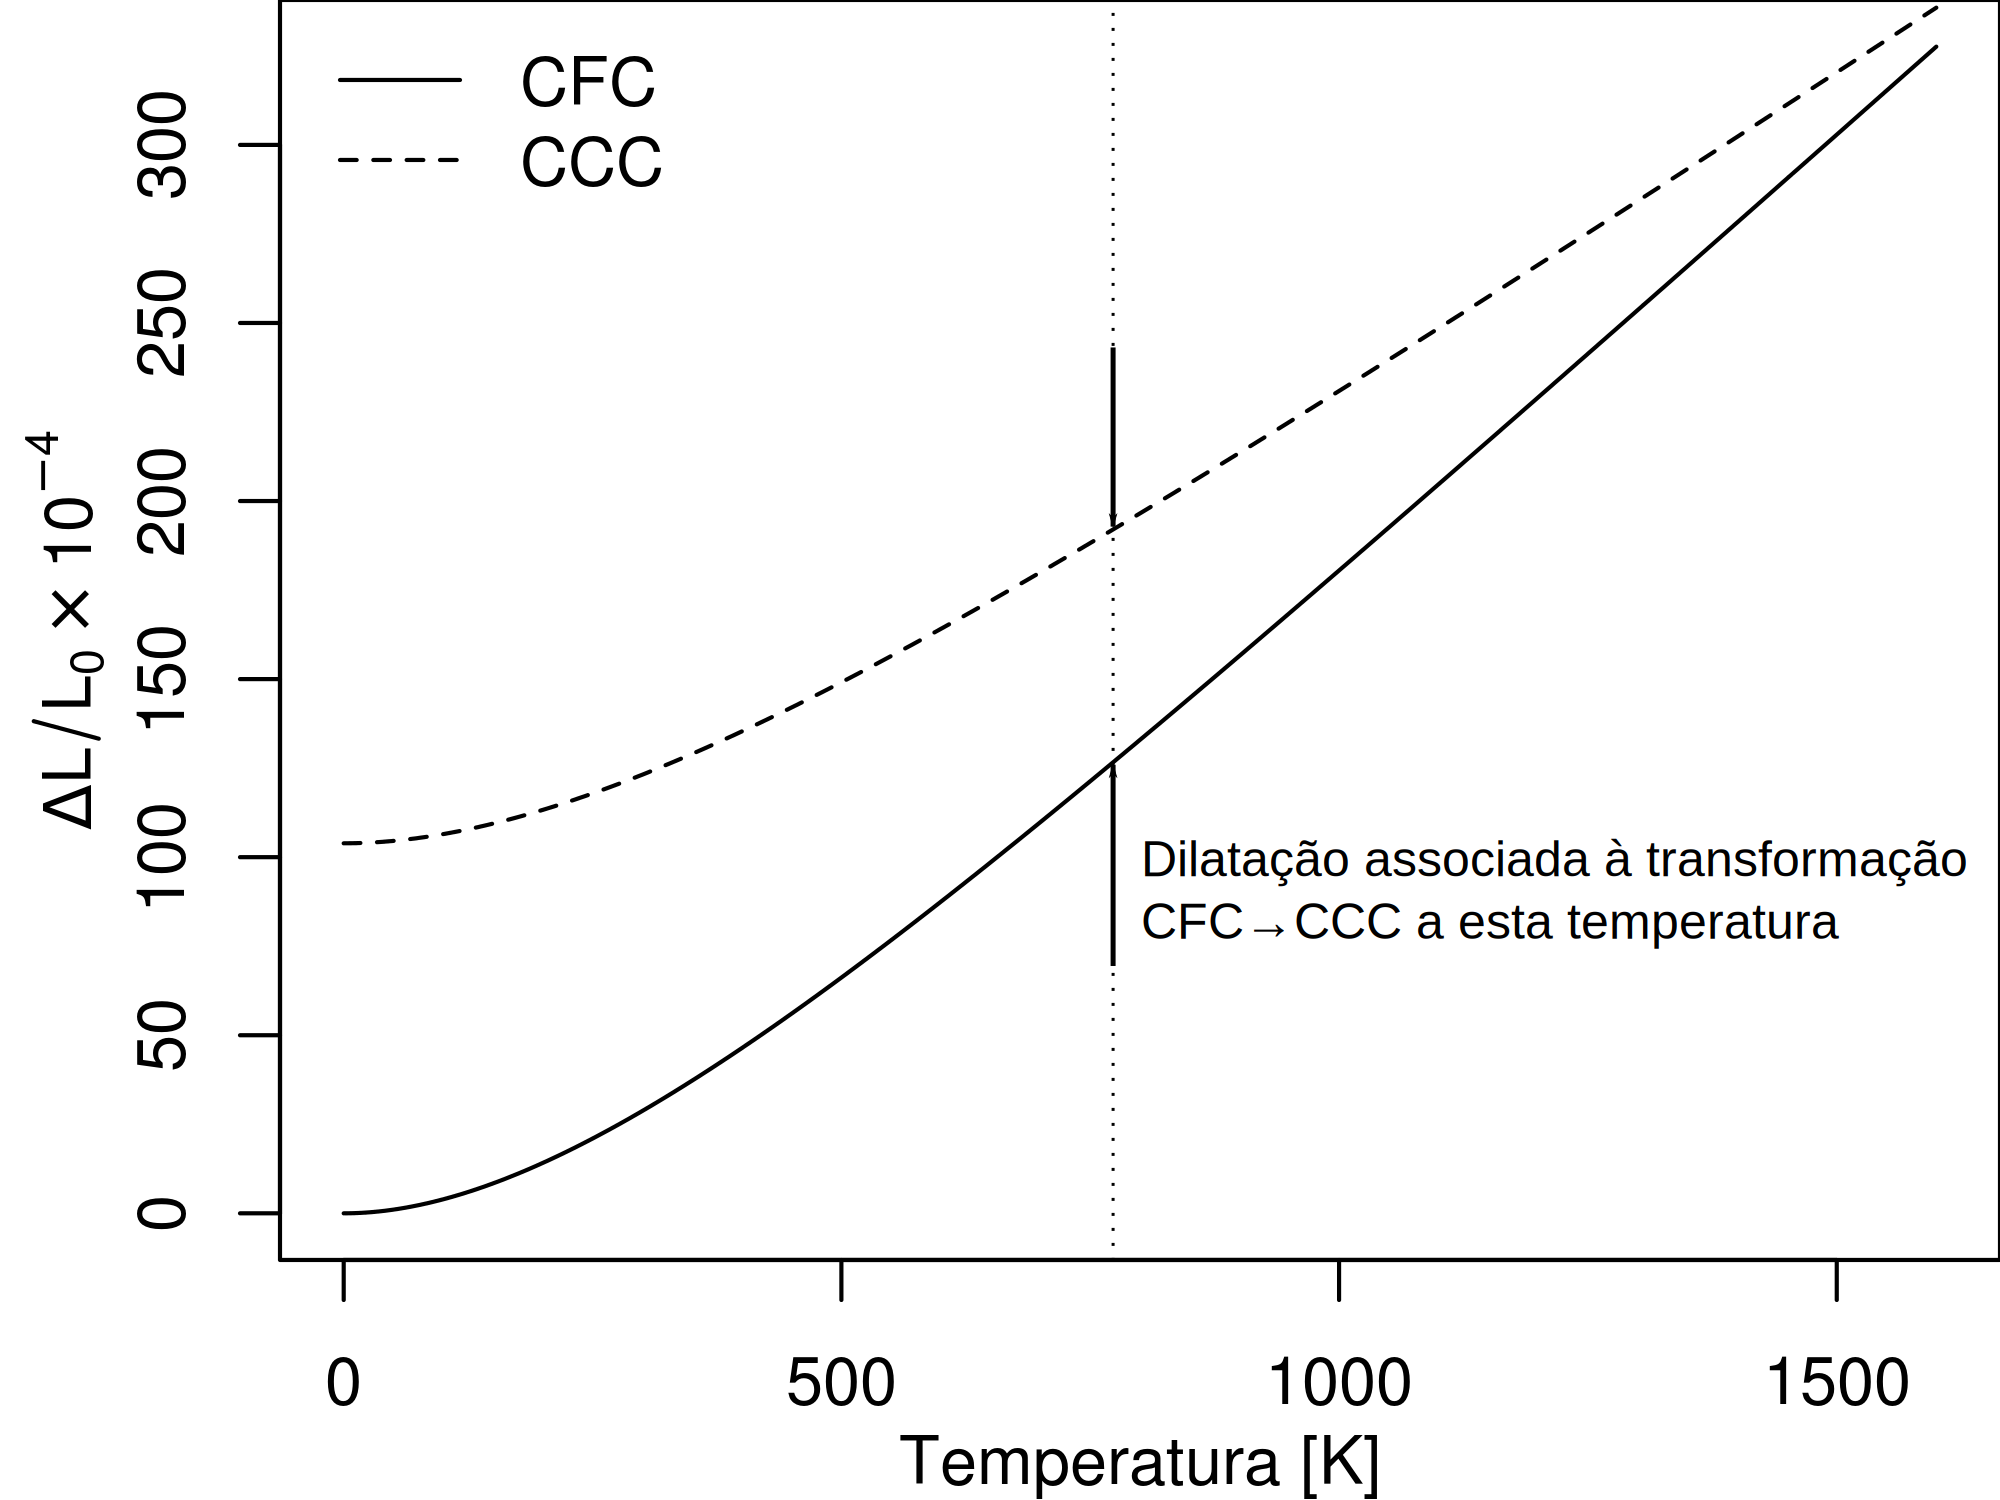
\includegraphics[width=12cm]{img/dilation_alphagamma.png}
	\caption{Dilatação térmica relativa ($\Delta L/L_0$) das fases cúbica de corpo centrado (CCC) e cúbica de corpo centrado (CFC). Curvas calculadas por meio das equações empíricas obtidas por\cite{VanBohemen2013b}.}
	\label{fig:dilRel}
\end{figure}

O tratamento de austêmpera da amostra tratada a 200 °C é essencialmente o mesmo aplicado no processo T\&P nas temperaturas de têmpera e partição de 200 °C. Nessa situação, a forte expansão observada no início do tratamento térmico é decorrente da transformação martensítica, haja vista esta temperatura de austêmpera é inferior à temperatura Ms. A dilatação subsequente, no entanto, não é completamente compatível com modelo JMAK e pode ser associada à partição de carbono da martensita para a austenita, precipitação de carbonetos no interior da martensita, ou mesmo a ocorrência da decomposição da austenita abaixo da temperatura Ms.

A amostra austemperada a 450 °C não apresentou contração durante a etapa isotérmica, ao contrário das amostras temperadas e particionadas na mesma temperatura. Dessa forma, descarta-se a hipótese de que a contração volumétrica nas amostras submetidas ao ciclo têmpera e partição a 450 °C esteja associada à reação bainítica durante a etapa de partição e devem estar associadas à precipitação de carbonetos no revenimento da martensita. Isso é compatível com a literatura sobre o assunto, que indica que tanto a precipitação de carbonetos de transição, quanto a precipitação da cementita levam à contração do material\cite{Morra2001}.

\section{Difra\c{c}\~{a}o de raios X \textit{in situ}}

\label{sec:DRXInSitu}

O mapa de cores da figura \ref{fig:colorMap} mostra a evolução dos padrões de difração ao etapa de partição da amostra temperada a 170 °C e particionada a 300 °C. Nesta figura as tonalidades representam a raiz quadrada da intensidade das reflexões do experimento de difração. É possível observar a evolução de diferentes picos associados ao obedecimento das condições de difração da austenita (fase $\gamma$) e da ferrita/martensita (fase $\alpha$).

\begin{figure}
	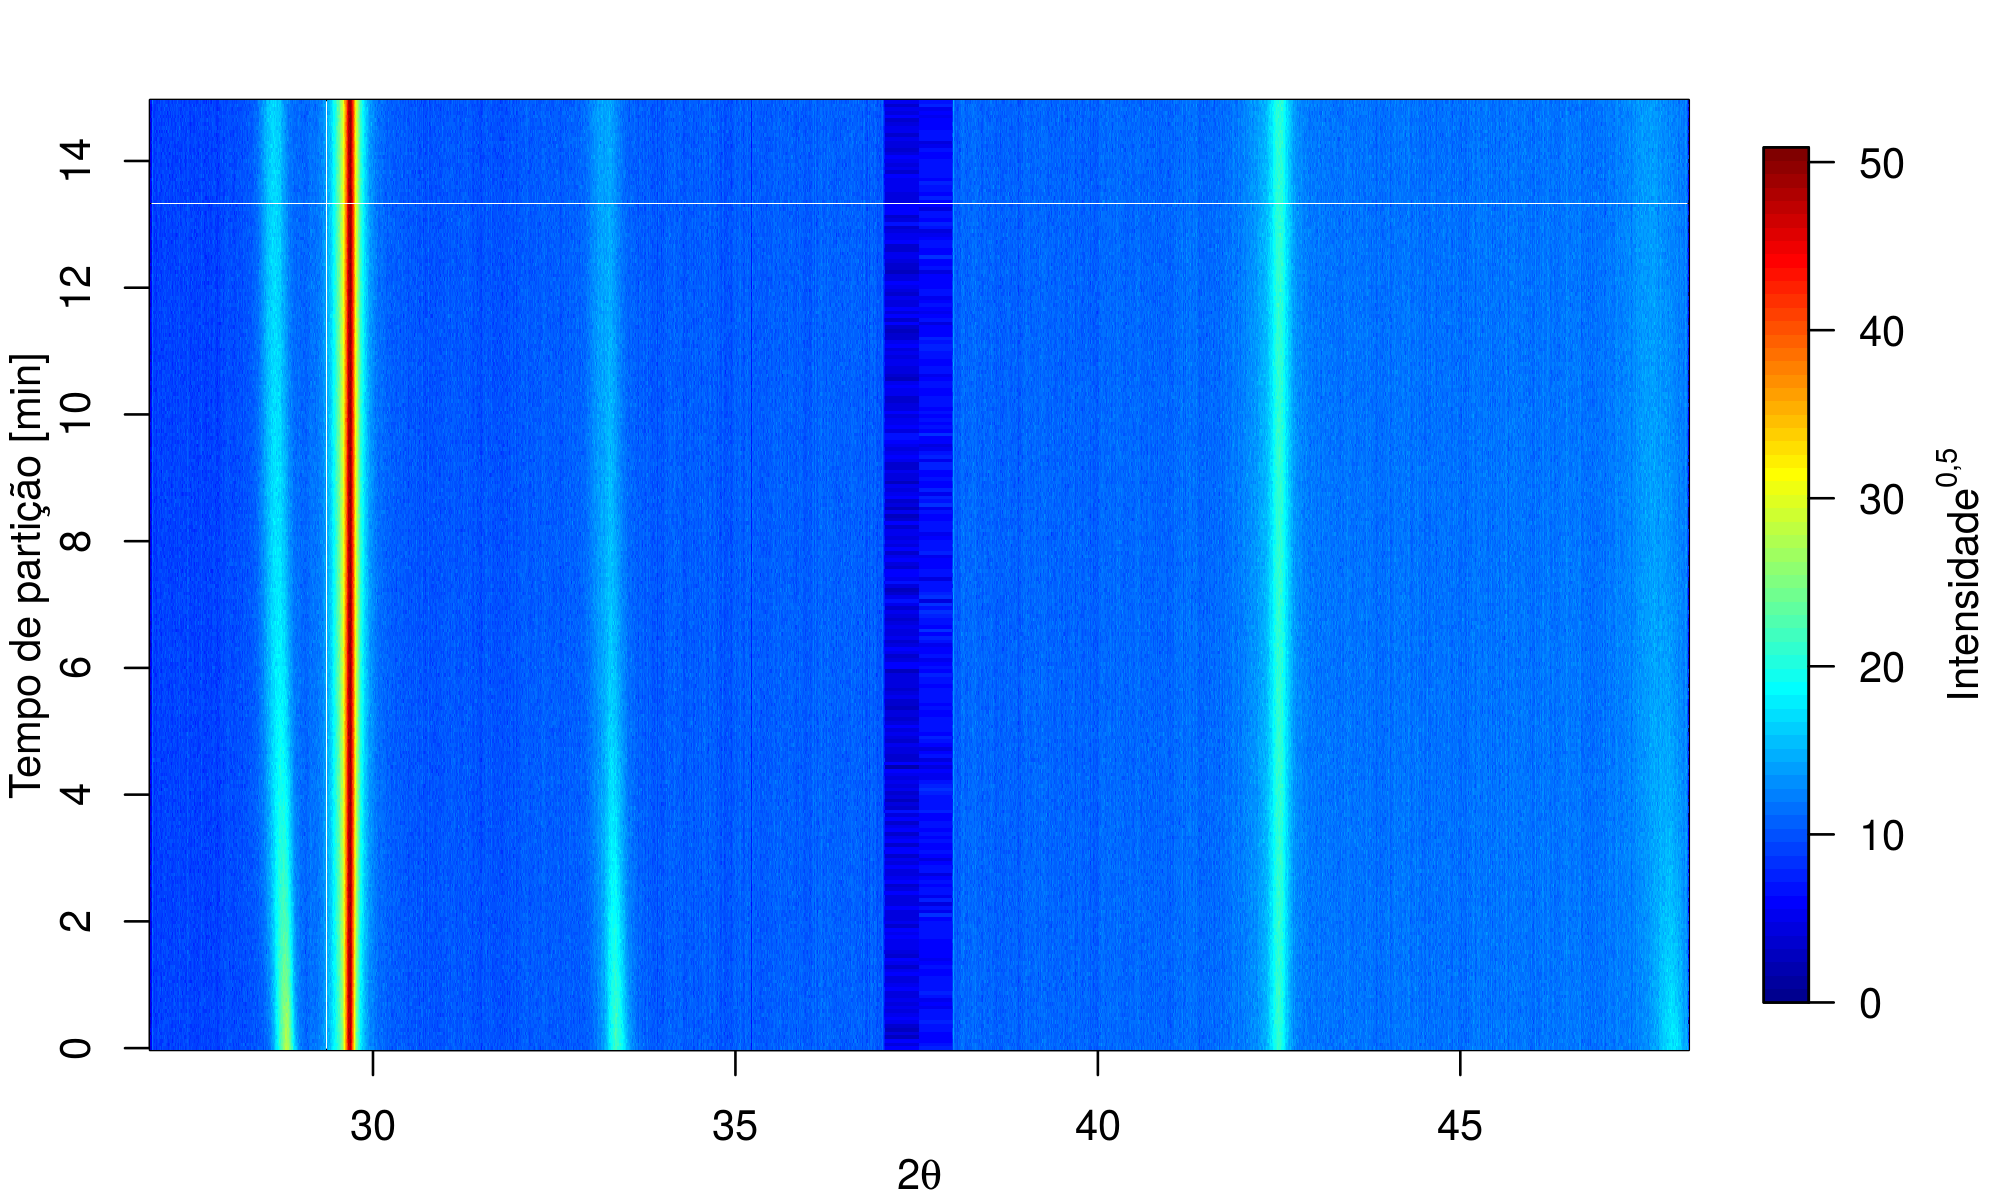
\includegraphics[width=16cm]{img/XTMS/map_TT170TP300.png}
	\caption{Mapa de cores representado a evolução dos picos de difração da austenita ($\gamma$) e da ferrita ($\alpha$) ao longo da etapa de partição. No eixo das abscissas é representado o ângulo de difração $2\theta$, enquanto no eixo das ordenadas é representado o tempo de partição em segundos. As tonalidades de cores correspondem à raiz quadrada da intensidade segundo a escala mostrado ao lado do mapa.}
	\label{fig:colorMap}
\end{figure}

Na figura \ref{fig:colorMap2} é possível ver em detalhe o mapa de cores da figura \ref{fig:colorMap}. É possível observar dois principais comportamentos: o deslocamento do pico {111} da austenita para ângulos menores de difração e sua diminuição de intensidade ao longo da etapa de partição. A lei de Bragg (equação \ref{eq:Bragg}) prevê que valores menores do ângulo $2\theta$ estão associados a maiores distâncias interplanares e, consequentemente, a maiores parâmetros de rede. Por sua vez, o aumento do parâmetro de rede é associado ao enriquecimento em carbono da austenita. A diminuição da intensidade do pico da austenita é interpretado pelo consumo da fase por uma reação competitiva, confirmando os resultados de dilatometria.

\begin{figure}
	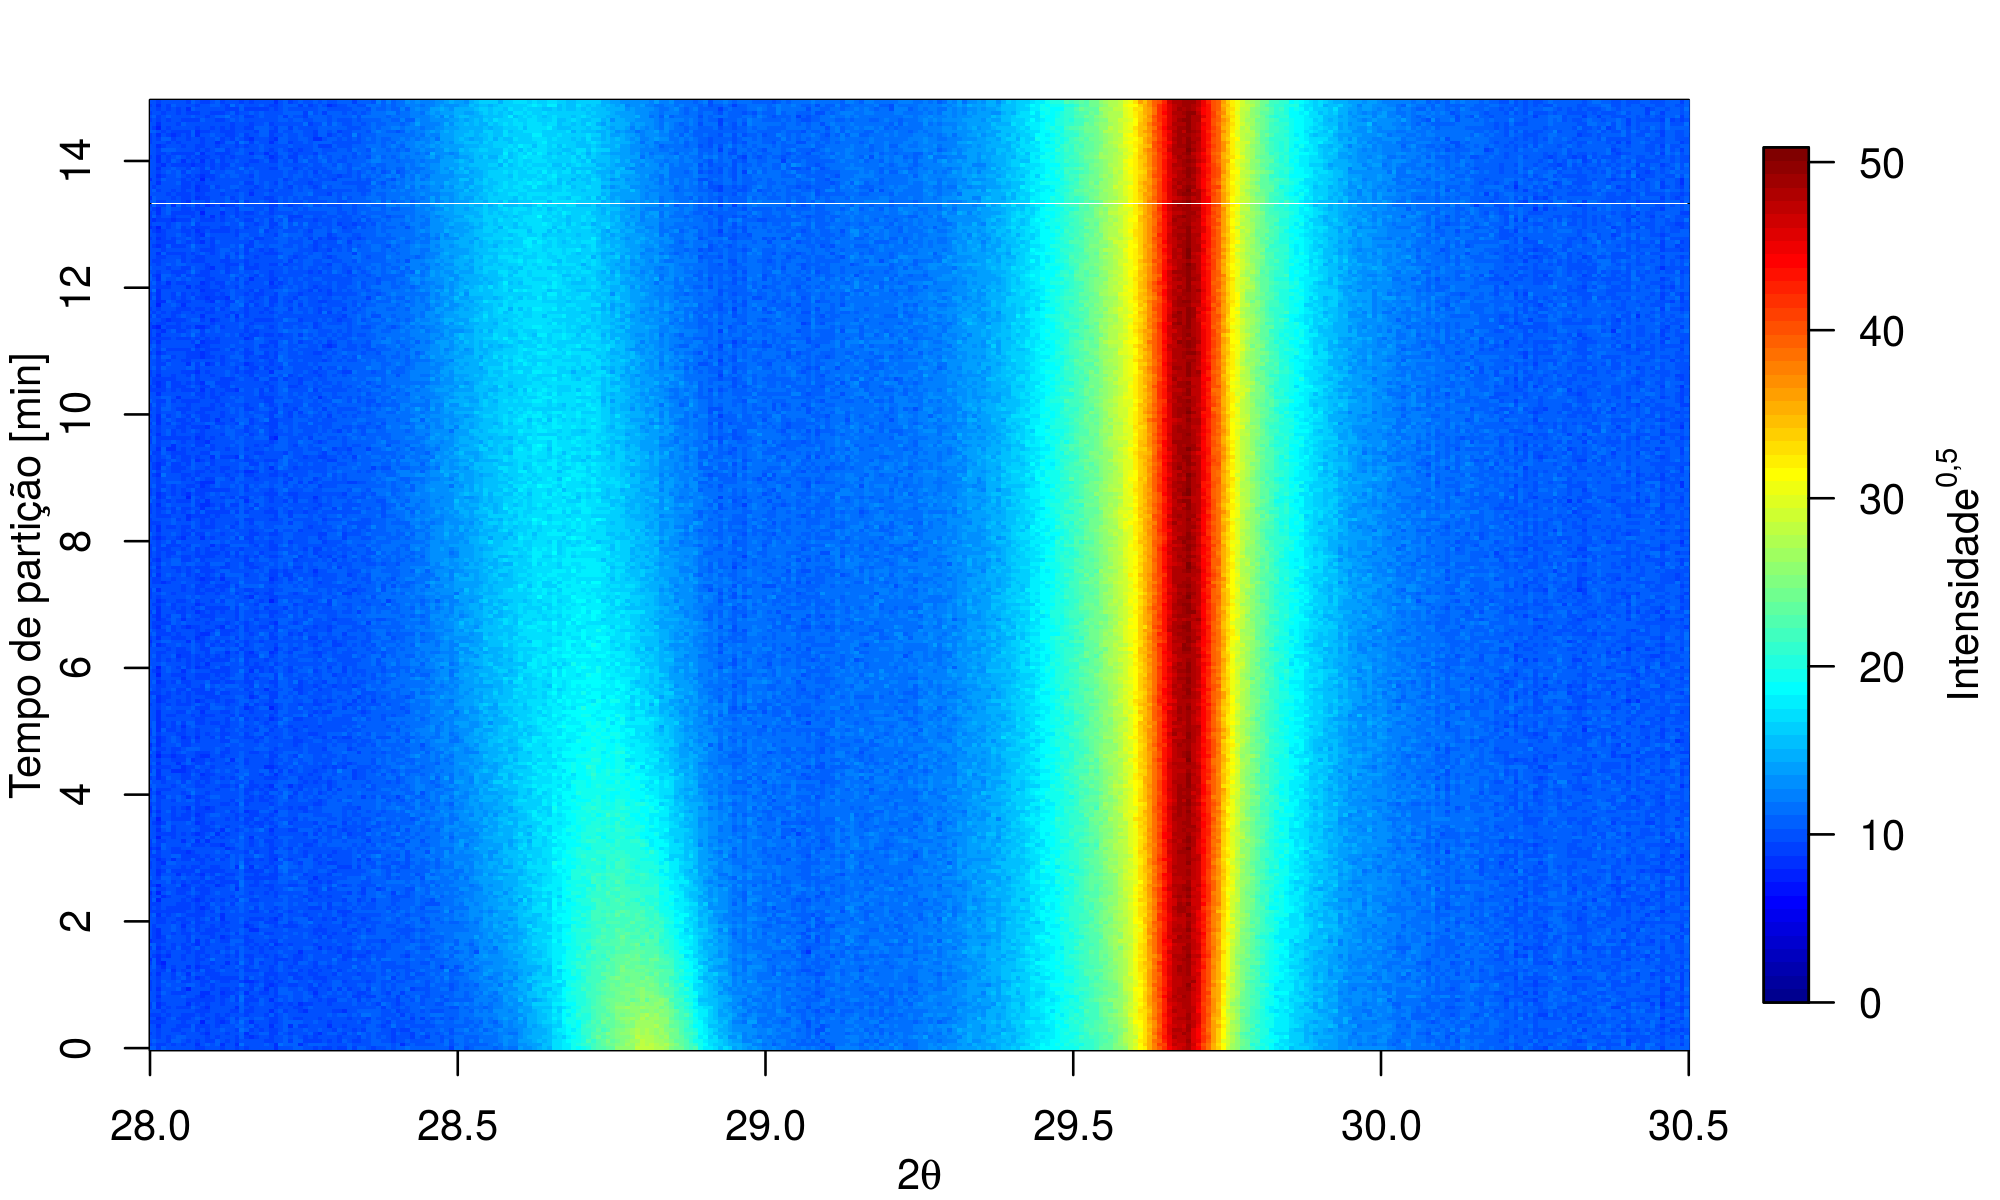
\includegraphics[width=16cm]{img/XTMS/map_TT170TP300_2.png}
	\caption{Detalhe do mapa de cores mostrado na figura \ref{fig:colorMap}.}
	\label{fig:colorMap2}
\end{figure}

As figuras \ref{fig:XTMSPT200} a \ref{fig:XTMSPT450} mostram os resultados de difração tratados para determinação da fração do produto isotérmico ($f^{\alpha\text{-iso}}$) formado durante a etapa de partição e a variação do teor de carbono dissolvido na austenita ($\Delta\%w_C^\gamma$), obtido pela relação de Dyson e Holmes (equação \ref{eq:parametroRede}).

\begin{figure}
	\subfloat[]{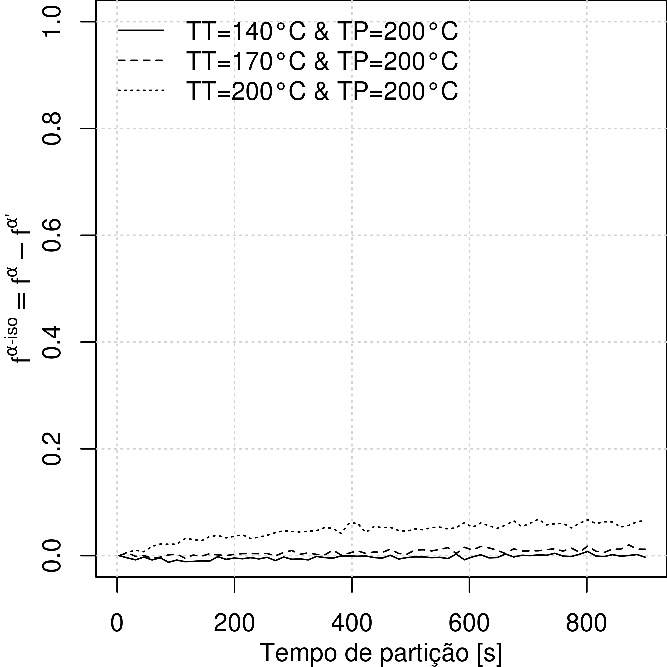
\includegraphics[width=7.5cm]{img/XTMS/f_isoPT200.png}}
	\quad
	\subfloat[]{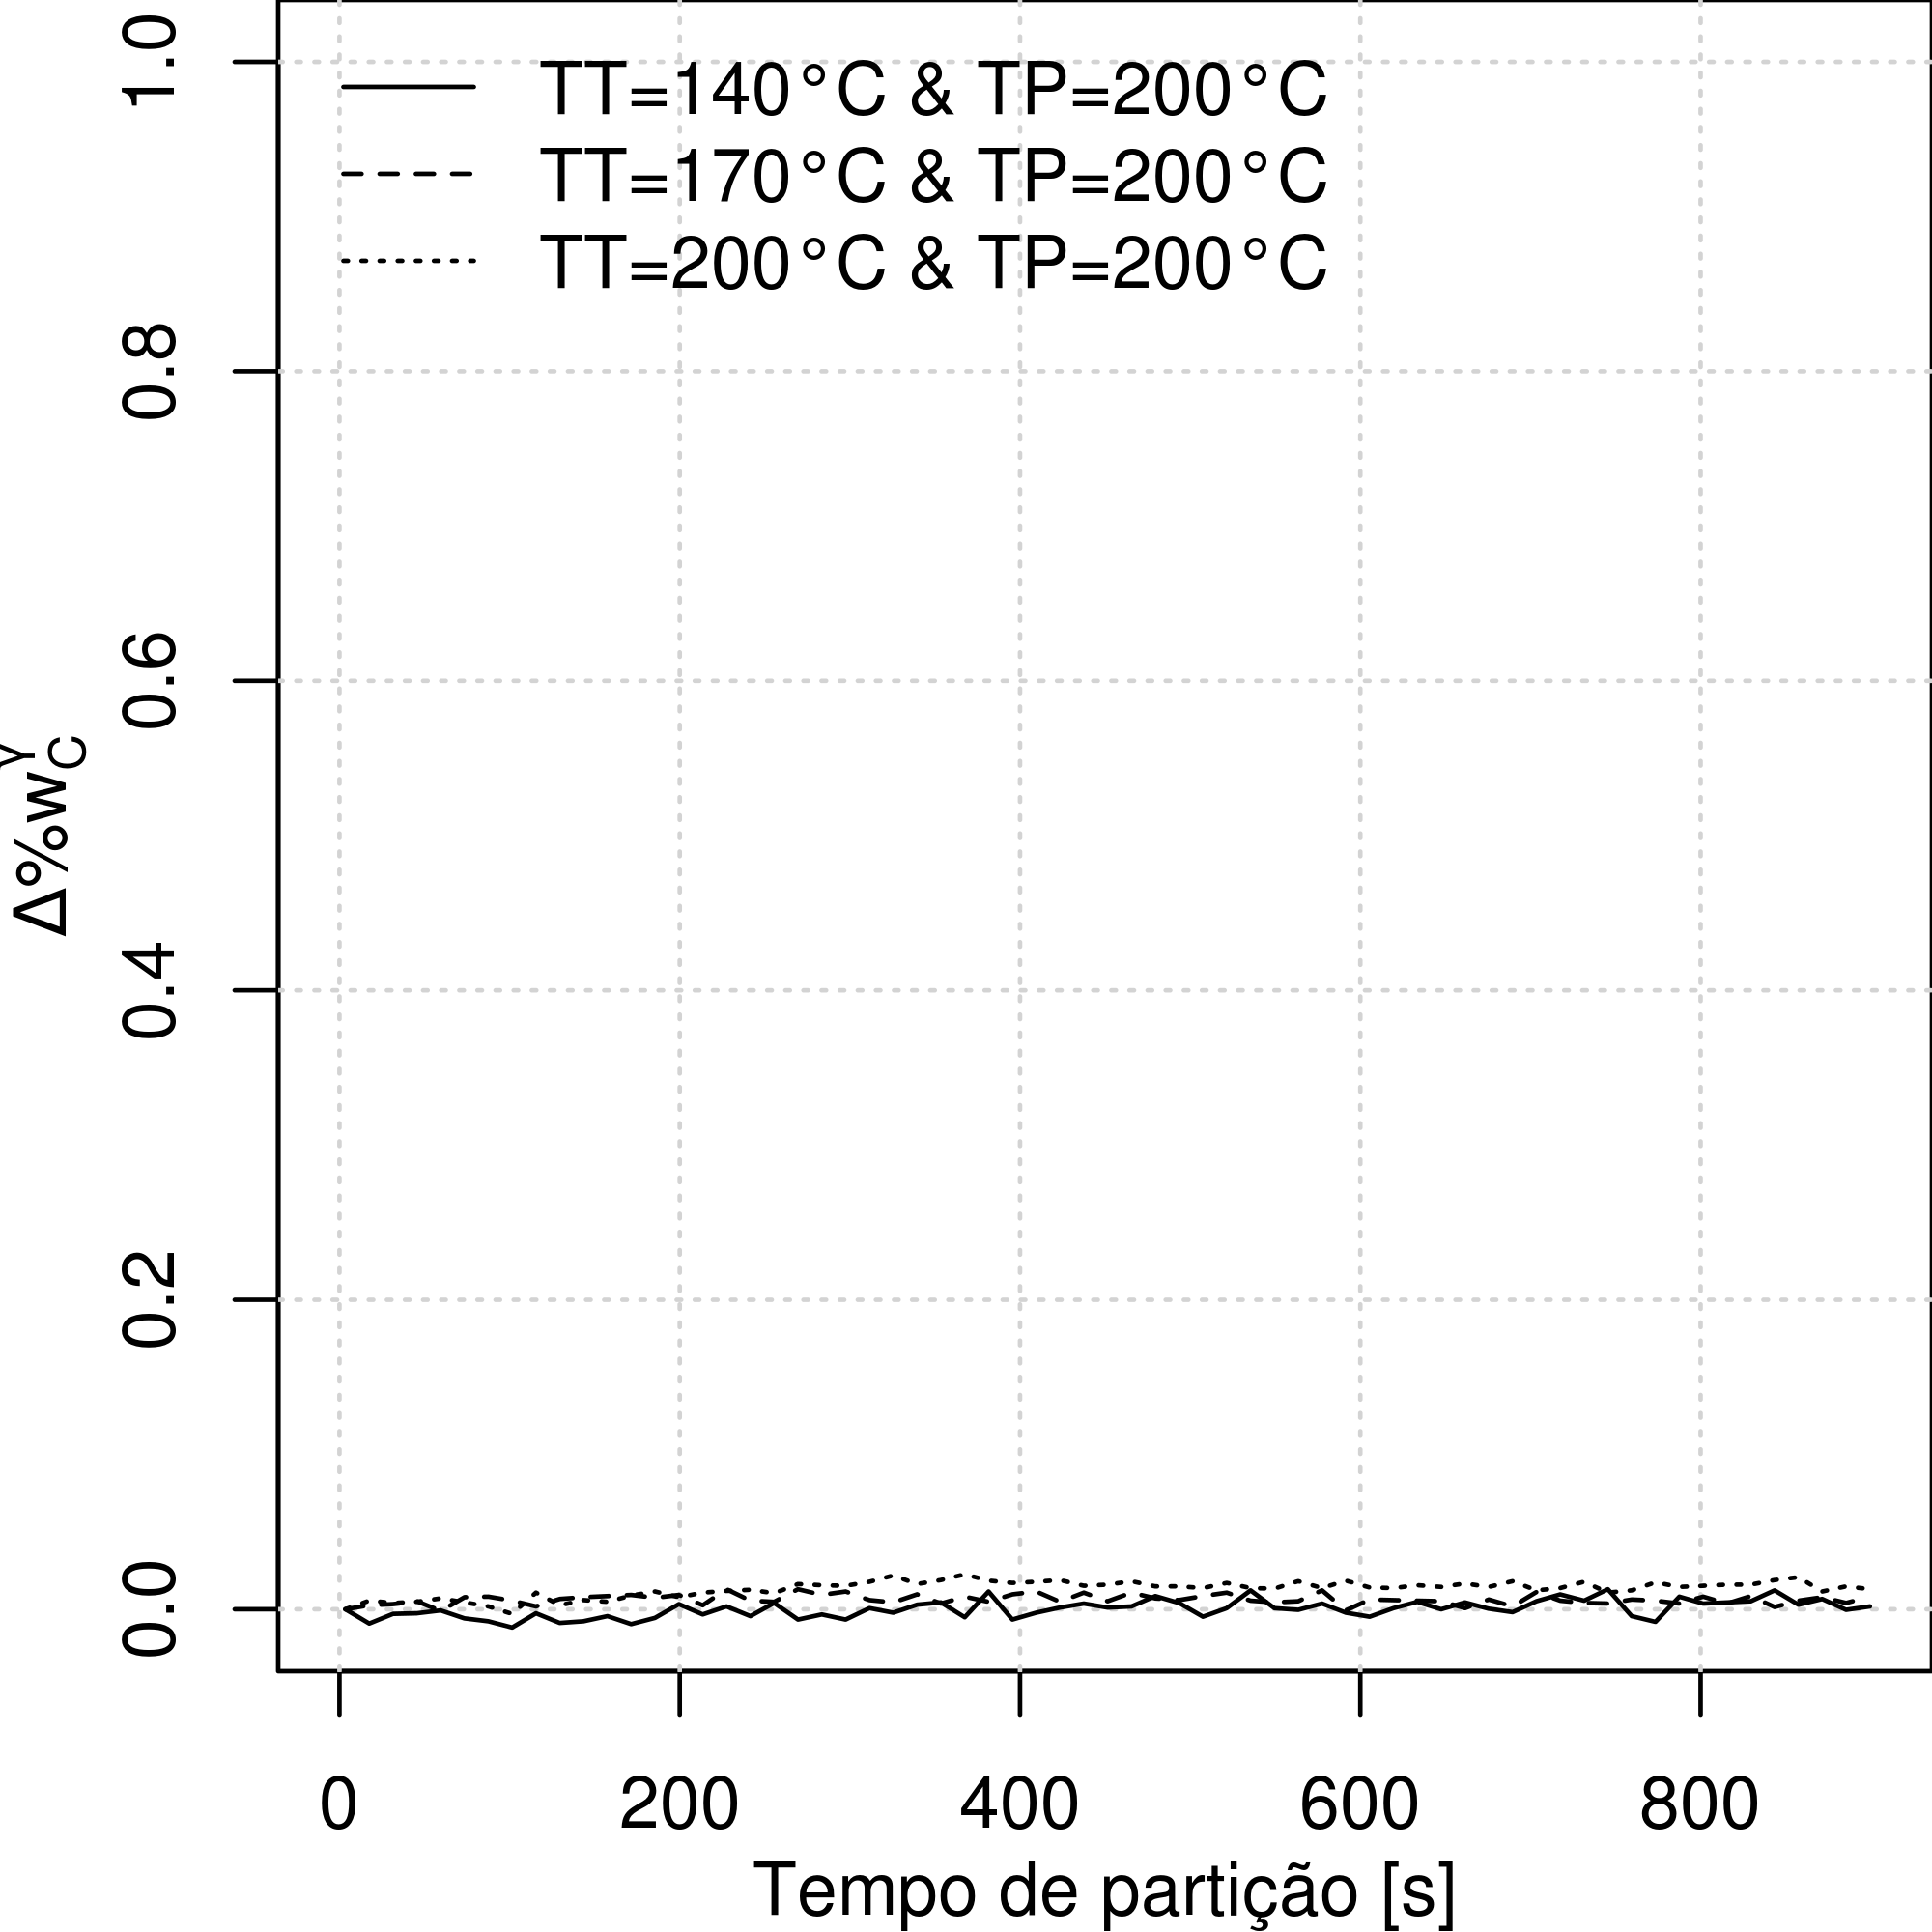
\includegraphics[width=7.5cm]{img/XTMS/wC_gamma200.png}}
	\caption{Fração volumétrica do produto isotérmico formado durante a partição (a) e teor de carbono dissolvido na austenita (b) para as amostradas particionadas a 200 °C.}
	\label{fig:XTMSPT200}
\end{figure}

\begin{figure}
	\subfloat[]{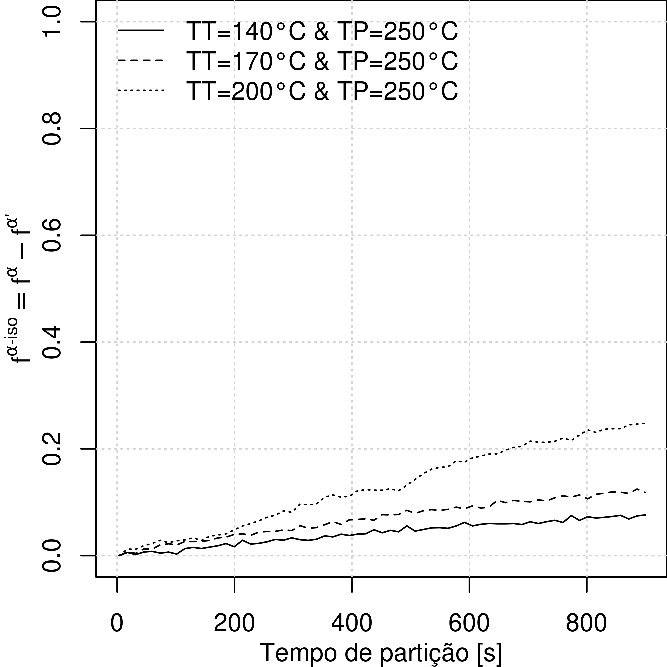
\includegraphics[width=7.5cm]{img/XTMS/f_isoPT250.png}}
	\quad
	\subfloat[]{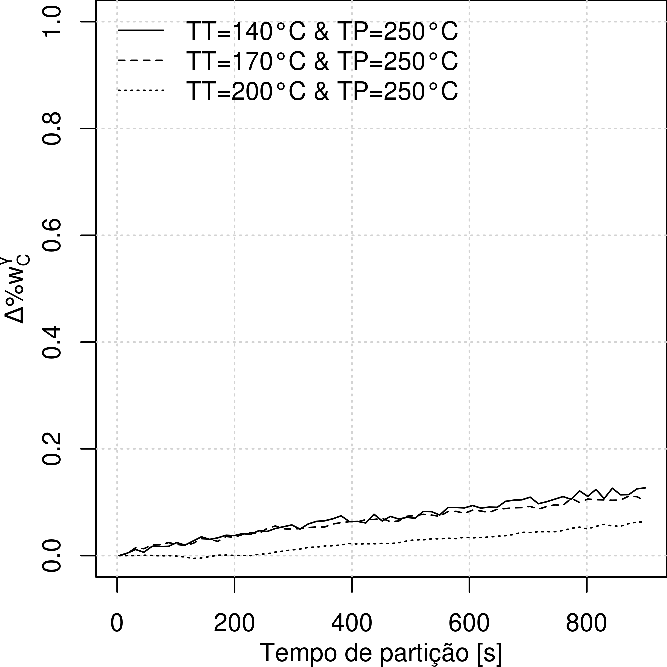
\includegraphics[width=7.5cm]{img/XTMS/wC_gamma250.png}}
	\caption{Fração volumétrica do produto isotérmico formado durante a partição (a) e teor de carbono dissolvido na austenita (b) para as amostradas particionadas a 250 °C.}
	\label{fig:XTMSPT250}
\end{figure}

\begin{figure}
	\subfloat[]{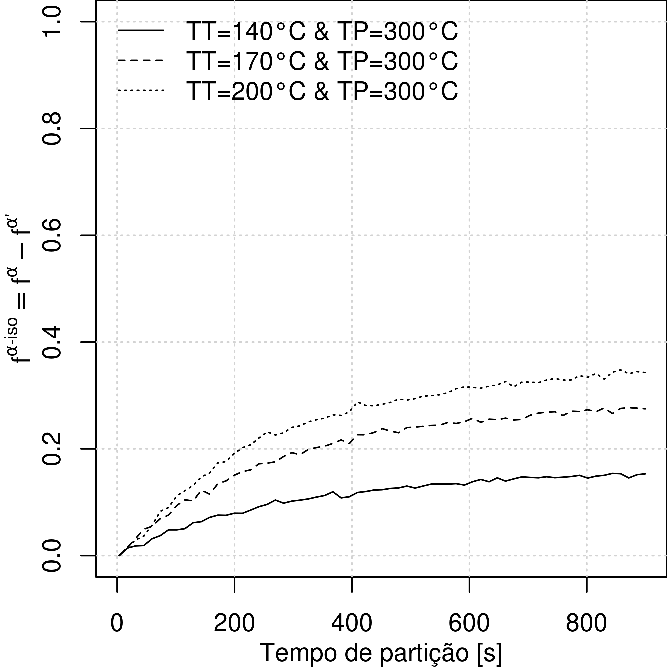
\includegraphics[width=7.5cm]{img/XTMS/f_isoPT300.png}}
	\quad
	\subfloat[]{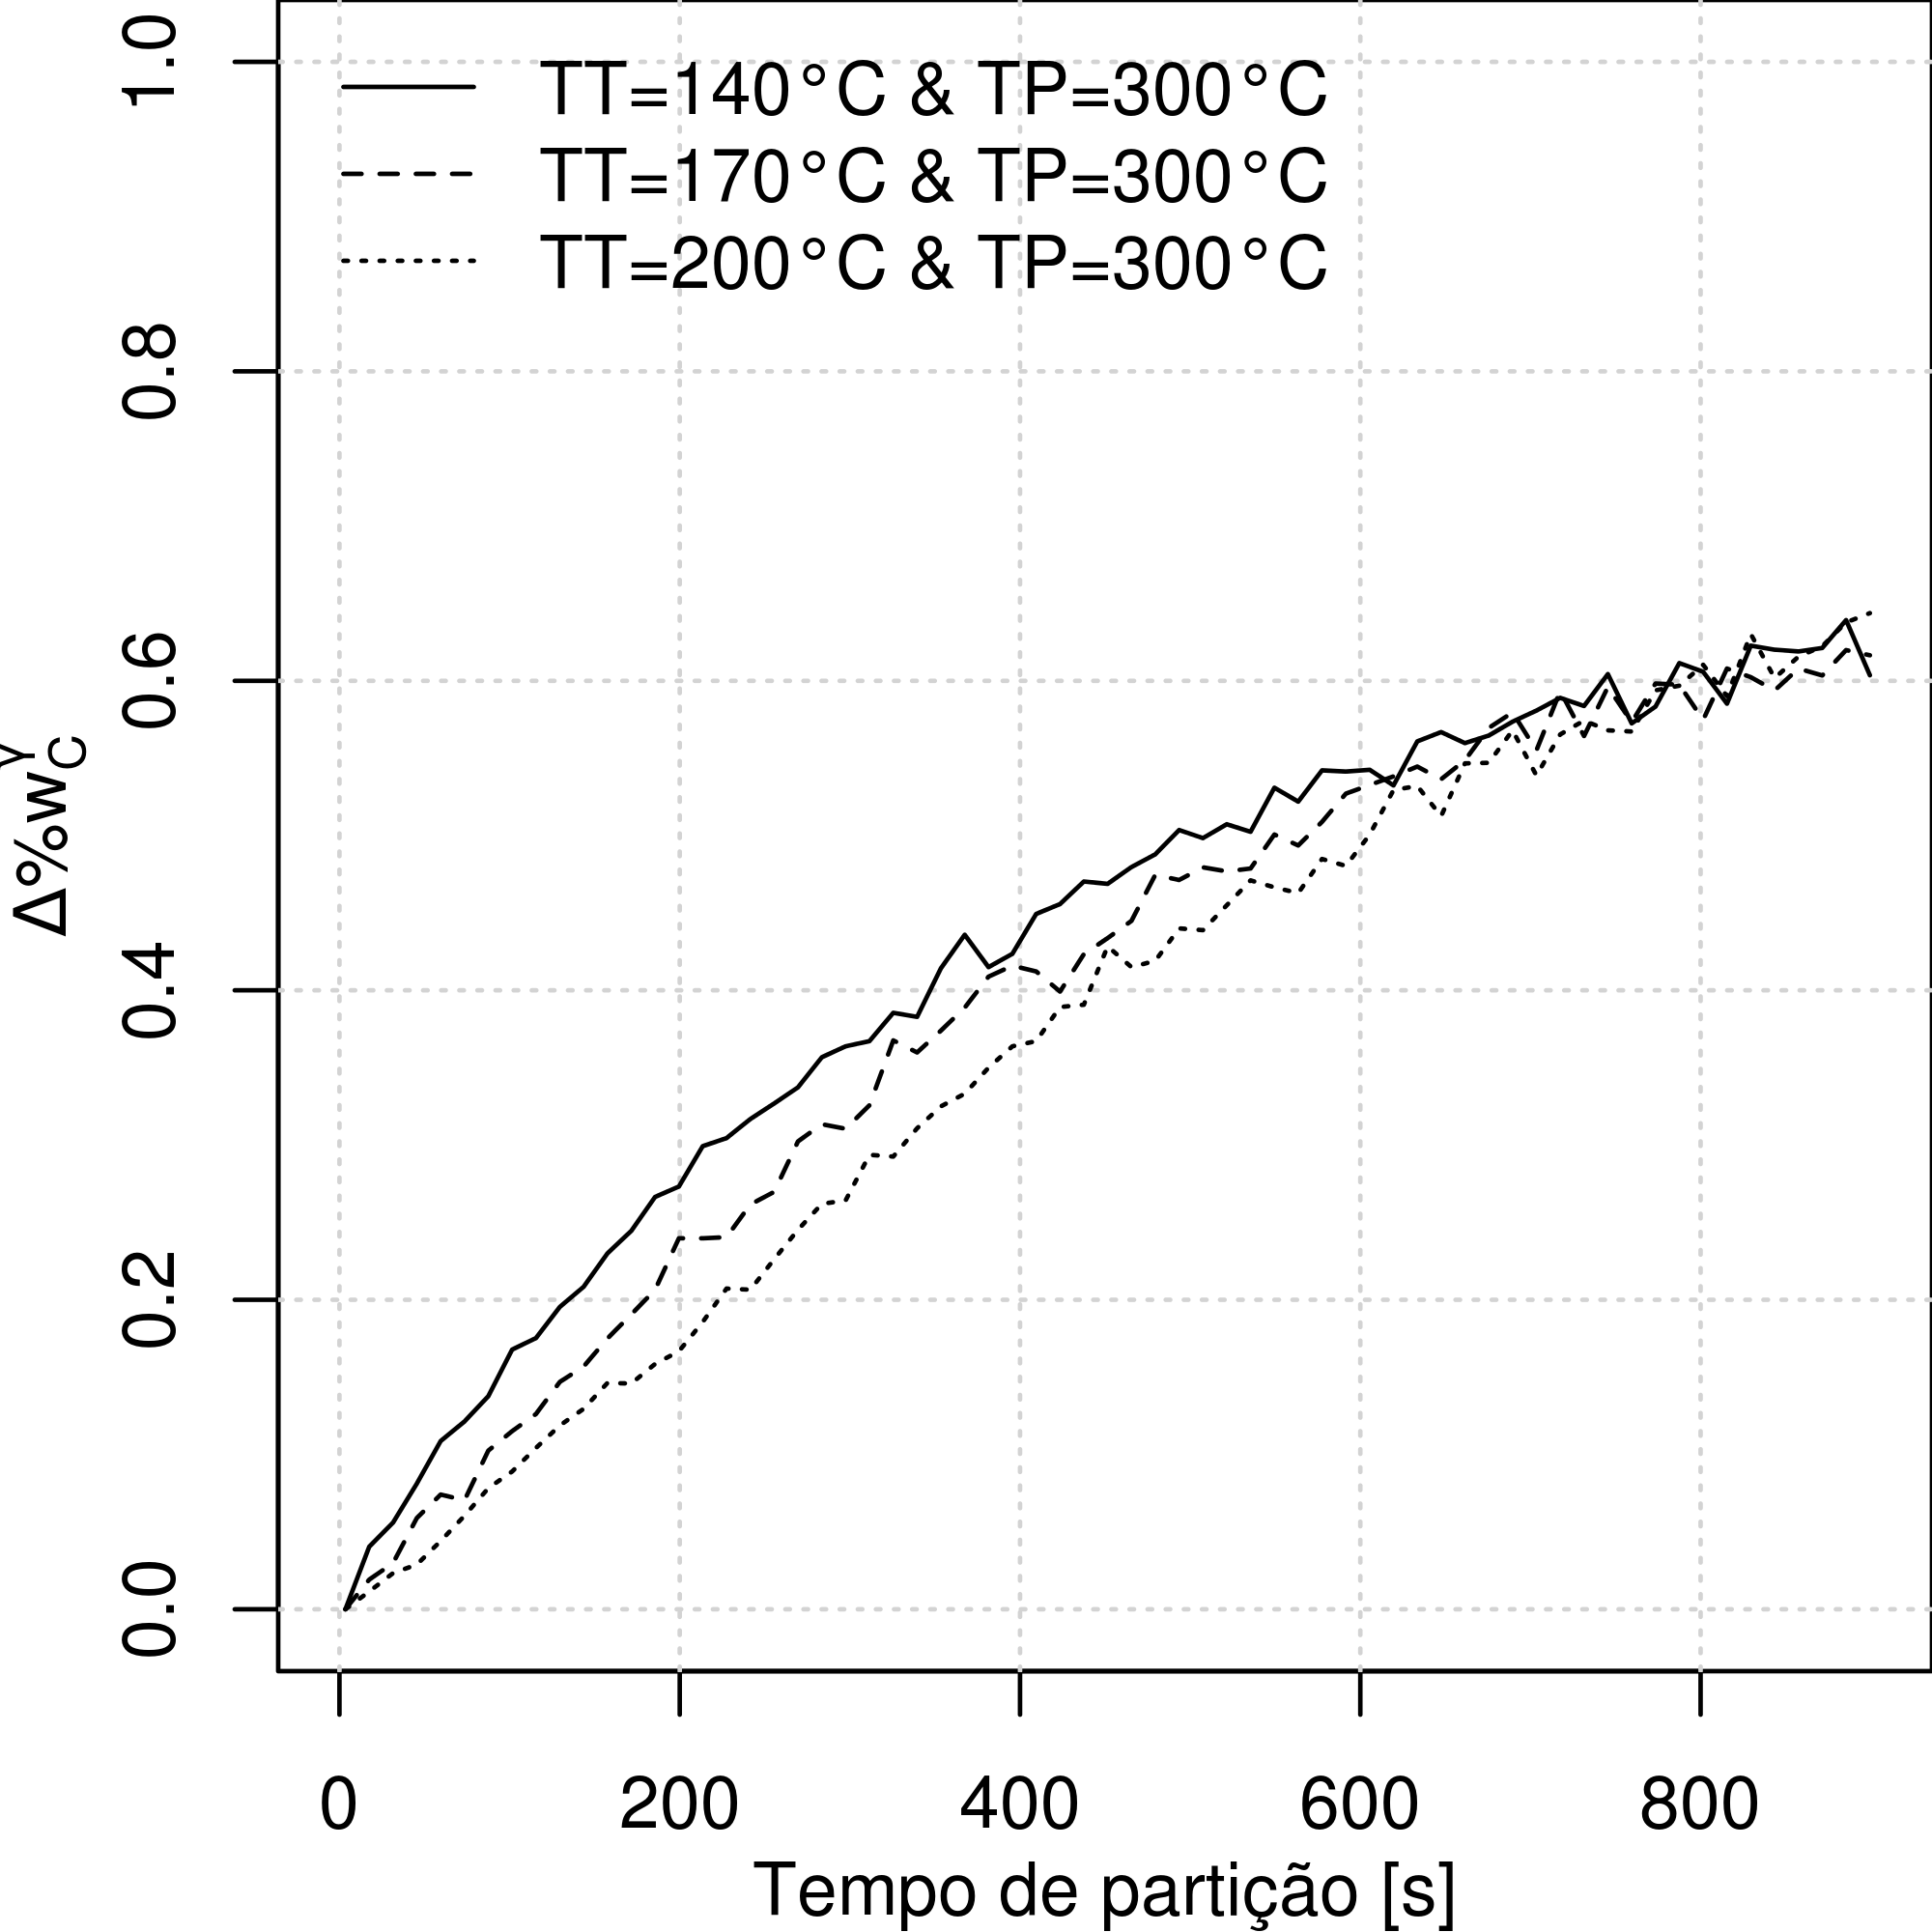
\includegraphics[width=7.5cm]{img/XTMS/wC_gamma300.png}}
	\caption{Fração volumétrica do produto isotérmico formado durante a partição (a) e teor de carbono dissolvido na austenita (b) para as amostradas particionadas a 300 °C.}
	\label{fig:XTMSPT300}
\end{figure}

\begin{figure}
	\subfloat[]{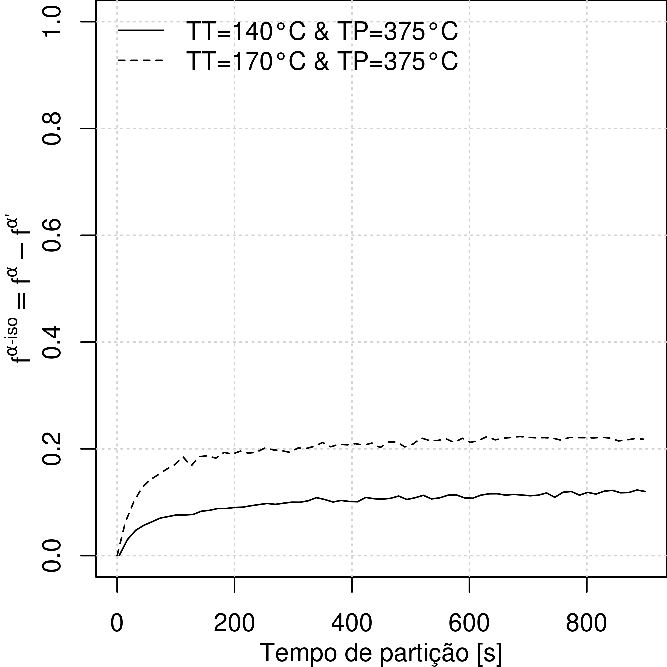
\includegraphics[width=7.5cm]{img/XTMS/f_isoPT375.png}}
	\quad
	\subfloat[]{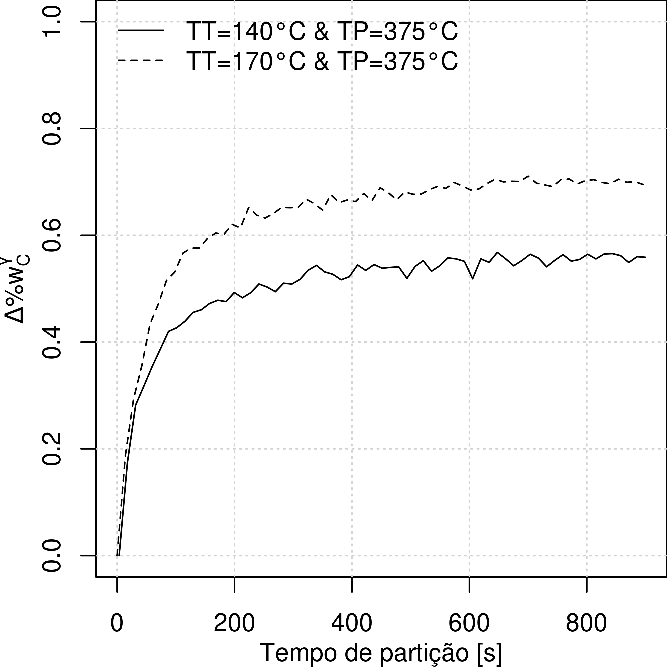
\includegraphics[width=7.5cm]{img/XTMS/wC_gamma375.png}}
	\caption{Fração volumétrica do produto isotérmico formado durante a partição (a) e teor de carbono dissolvido na austenita (b) para as amostradas particionadas a 375 °C.}
	\label{fig:XTMSPT375}
\end{figure}

\begin{figure}
	\subfloat[]{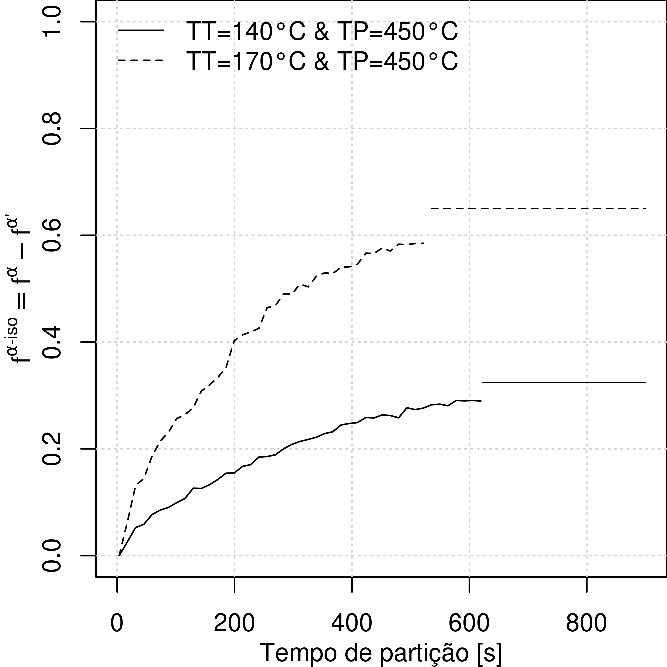
\includegraphics[width=7.5cm]{img/XTMS/f_isoPT450.png}}
	\quad
	\subfloat[]{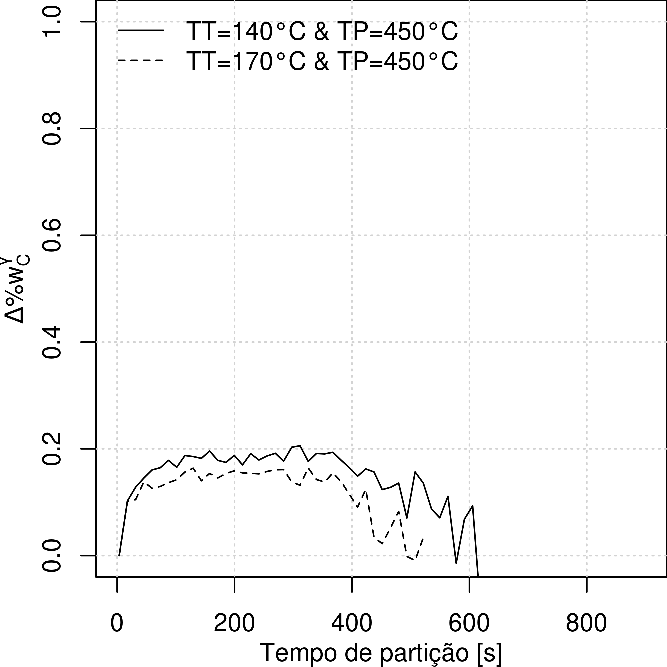
\includegraphics[width=7.5cm]{img/XTMS/wC_gamma450.png}}
	\caption{Fração volumétrica do produto isotérmico formado durante a partição (a) e teor de carbono dissolvido na austenita (b) para as amostradas particionadas a 450 °C.}
	\label{fig:XTMSPT450}
\end{figure}

Observam-se comportamentos semelhantes aos constatados nos resultados de dilatometria. Nota-se que, dentre as amostras particionadas a 200 °C, há, de fato, a formação de uma pequena quantidade do produto $\alpha\text{-iso}$ na amostra temperada a 200 °C(figura \ref{fig:XTMSPT200}a). No entanto, o enriquecimento em carbono da austenita é praticamente imperceptível pela análise das curvas da figura \ref{fig:XTMSPT200}b. Esse resultado vai contra a observação feita pelos resultados de dilatometria de que mesmo nas condições partição a 200 °C a temperatura Ms diminui consideravelmente (vide tabela \ref{tab:MsTP}).

Nas demais condições de tratamento térmico também é possível observar substancial aumento da fração volumétrica da fase cúbica de corpo centrado ($\alpha$) e consequente diminuição da fração volumétrica da austenita não transformada. Confirmando os resultados apontados pela dilatometria, maiores temperaturas de têmpera produziram maiores frações do produto isotérmico. Em contrapartida, com exceção das amostras particionadas a 450 °C, o enriquecimento em carbono da austenita também é significativo. Além disso, o comportamento das curvas de variação do carbono na austenita é bastante similar às curvas de fração transformada. Isso leva à conclusão de que a formação do produto isotérmico $\alpha\text{-iso}$ contribui fortemente para o enriquecimento em carbono e estabilização da austenita.

Nas amostras particionadas a 300 °C, após os 15 minutos da etapa de partição todas as condições de têmpera produziram aproximadamente o mesmo acréscimo no teor de carbono de austenita, cerca de 0,6\% (figura \ref{fig:XTMSPT300}b). O que se mostra diferente entre as três diferentes condições de têmpera é o comportamento cinético nos primeiros segundos da etapa de partição: a amostra temperada a 140 °C leva ao enriquecimento em carbono da austenita de forma mais rápida do que nas demais condições. Esse resultado complementa a análise feita com os resultados de dilatometria. Parece razoável concluir que a quantidade de martensita formada durante a etapa de têmpera --- tão maior, quanto menor a temperatura de têmpera --- desempenha papel fundamental na cinética da reação isotérmica.

As amostras particionadas a 375 °C não apresentam a mesma convergência do teor de carbono na austenita após a etapa de partição. A condição de têmpera a 170 °C produziu cerca de 0,7\% de acréscimo no teor de carbono da austenita, contra 0,6\% obtido para a amostra temperada a 140 °C. Nessa situação, diferenças no comportamento cinético não foram observadas.

Nas amostras tratadas a 450 °C observa-se uma descontinuidade nas curvas de fração transformada (figura \ref{fig:XTMSPT450}a). Isto é consequente da dificuldade da rotina numérica quantificar as quantidades muito pequenas de austenita restantes no final da etapa de partição. Esta foi a única condição de partição que levou ao consumo completo da austenita ao final da etapa de partição. Por este motivo, o teor de carbono dissolvido na austenita gerou resultados bastante ruidosos para os instantes finais de partição (figura \ref{fig:XTMSPT450}b). Dessa forma, embora se observe uma aparente diminuição no teor de carbono da austenita ao final da partição, esta conclusão pode estar sendo prejudicada pelo método de medição em si.

\subsection{Carbono dissolvido na martensita particionada/ferrita formada isotermicamente}

\label{subsec:wCalpha}

Assumindo que as únicas fases presente na matriz do ferro fundido são a austenita $\gamma$ e a martensita particionada/ferrita isotérmica $\alpha$, o teor de carbono médio dissolvido na fase $\alpha$ pode ser determinado a partir dos resultados de DRX utilizando as equações de balanço de massa de carbono e de balanço das quantidades das fases:

\begin{subequations}
	\begin{align}
		&\%w_C^\alpha \cdot f^\alpha + \%w_C^\gamma \cdot f^\gamma = \%w_C^0\\
		&f^\alpha + f^\gamma = 1 
	\end{align}
	\label{eq:wCalpha}
\end{subequations}
%
em que $w_C^\alpha$ e $w_C^\gamma$ são as porcentagens em massa de carbono dissolvido nas fases $\alpha$ e $\gamma$, respectivamente, $w_C^0$ é o teor de carbono inicial dissolvido na austenita e $f^\alpha$ e $f^\gamma$ são as frações volumétricas de $\alpha$ e $\gamma$. A partir das equações acima e, assumindo o teor de carbono inicial da austenita determinado pelos cálculos termodinâmicos pelo Thermo-Calc\textregistered{} (0,76\%, segundo a tabela \ref{tab:CQaust}, a evolução do teor de carbono na ferrita/martensita ao longo da etapa de partição foi determinada para cada condição estudada, sendo mostrada na figura \ref{fig:wCalpha}.

\begin{figure}
	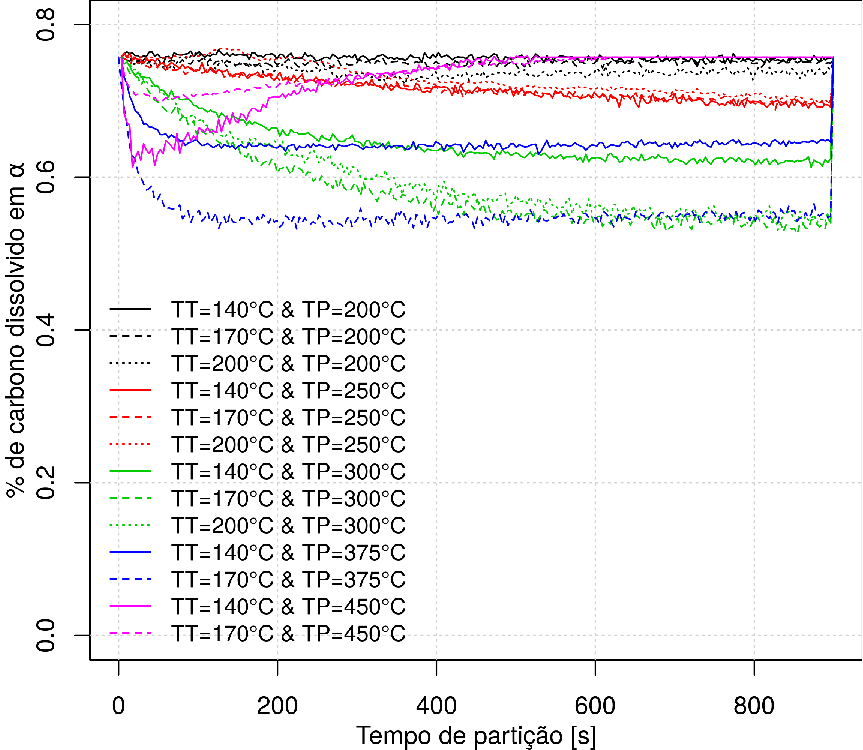
\includegraphics[width=12cm]{img/XTMS/wC_alpha.png}
	\caption{Teor de carbono dissolvido na ferrita/martensita em função do tempo de partição.}
	\label{fig:wCalpha}
\end{figure}

Nota-se que nas condições de partição a 450 °C há uma inicial diminuição do carbono na fase $\alpha$, seguida de um rápido aumento, até o reestabelecimento da fração inicial de carbono. Esse resultado é incompatível com a segunda lei da termodinâmica, pois o enriquecimento em carbono da ferrita ao longo de um tratamento isotérmico provocaria o aumento da energia livre do sistema. O que acontece nesta situação é que, como as equações \ref{eq:wCalpha} não incorporam no balanço de massa a presença de uma terceira fase, a precipitação de uma terceira fase rica em carbono levaria a esse tipo de distorção dos resultados. Dessa forma, o acréscimo do teor de carbono observado para a fase $\alpha$ é provavelmente decorrente da precipitação de cementita no segundo estágio da reação baínitica durante a etapa de partição.

Nas demais condições de partição não são observadas inversões de tendências para o carbono dissolvido em $\alpha$. É possível observar que em todos os casos ocorre o empobrecimento monotônico do carbono médio. No entanto, em nenhum caso o teor de carbono figurou abaixo de 0,5\%. Essa composição é correspondente à de martensita de médio carbono e, portanto, conclui-se que nem todo o potencial de enriquecimento da austenita foi atingido. Este teor de carbono dissolvido em $\alpha$ pode ser justificado ou pela permanência da supersaturação de carbono na martensita mesmo após a etapa de partição, ou pela precipitação de carbonetos de revenimento na martensita.

Face a essas observações, formula-se a hipótese de que o principal mecanismo de enriquecimento em carbono da austenita nas amostras temperadas e particionadas é, de fato, a reação isotérmica durante a etapa de partição e que a partição de carbono da martensita para a austenita é mínima, ou não chega a ocorrer, prevalecendo a supersaturação da martensita, ou a precipitação de carbonetos de revenimento.

\subsection{Quantidades finais de austenita após o resfriamento final}

A figura \ref{fig:finalScan} mostra o difratograma obtido após o resfriamento final da amostra temperada a 170 °C e particionada a 300 °C. Os picos de difração indexados das fases $\alpha$ e $\gamma$ foram utilizados para quantificar a fração de austenita retida. A tabela \ref{tab:fracGamma} sumariza as quantidades de austenita retida e as variações de carbono na austenita produzidas para cada condição de tratamento térmico.

\begin{figure}
	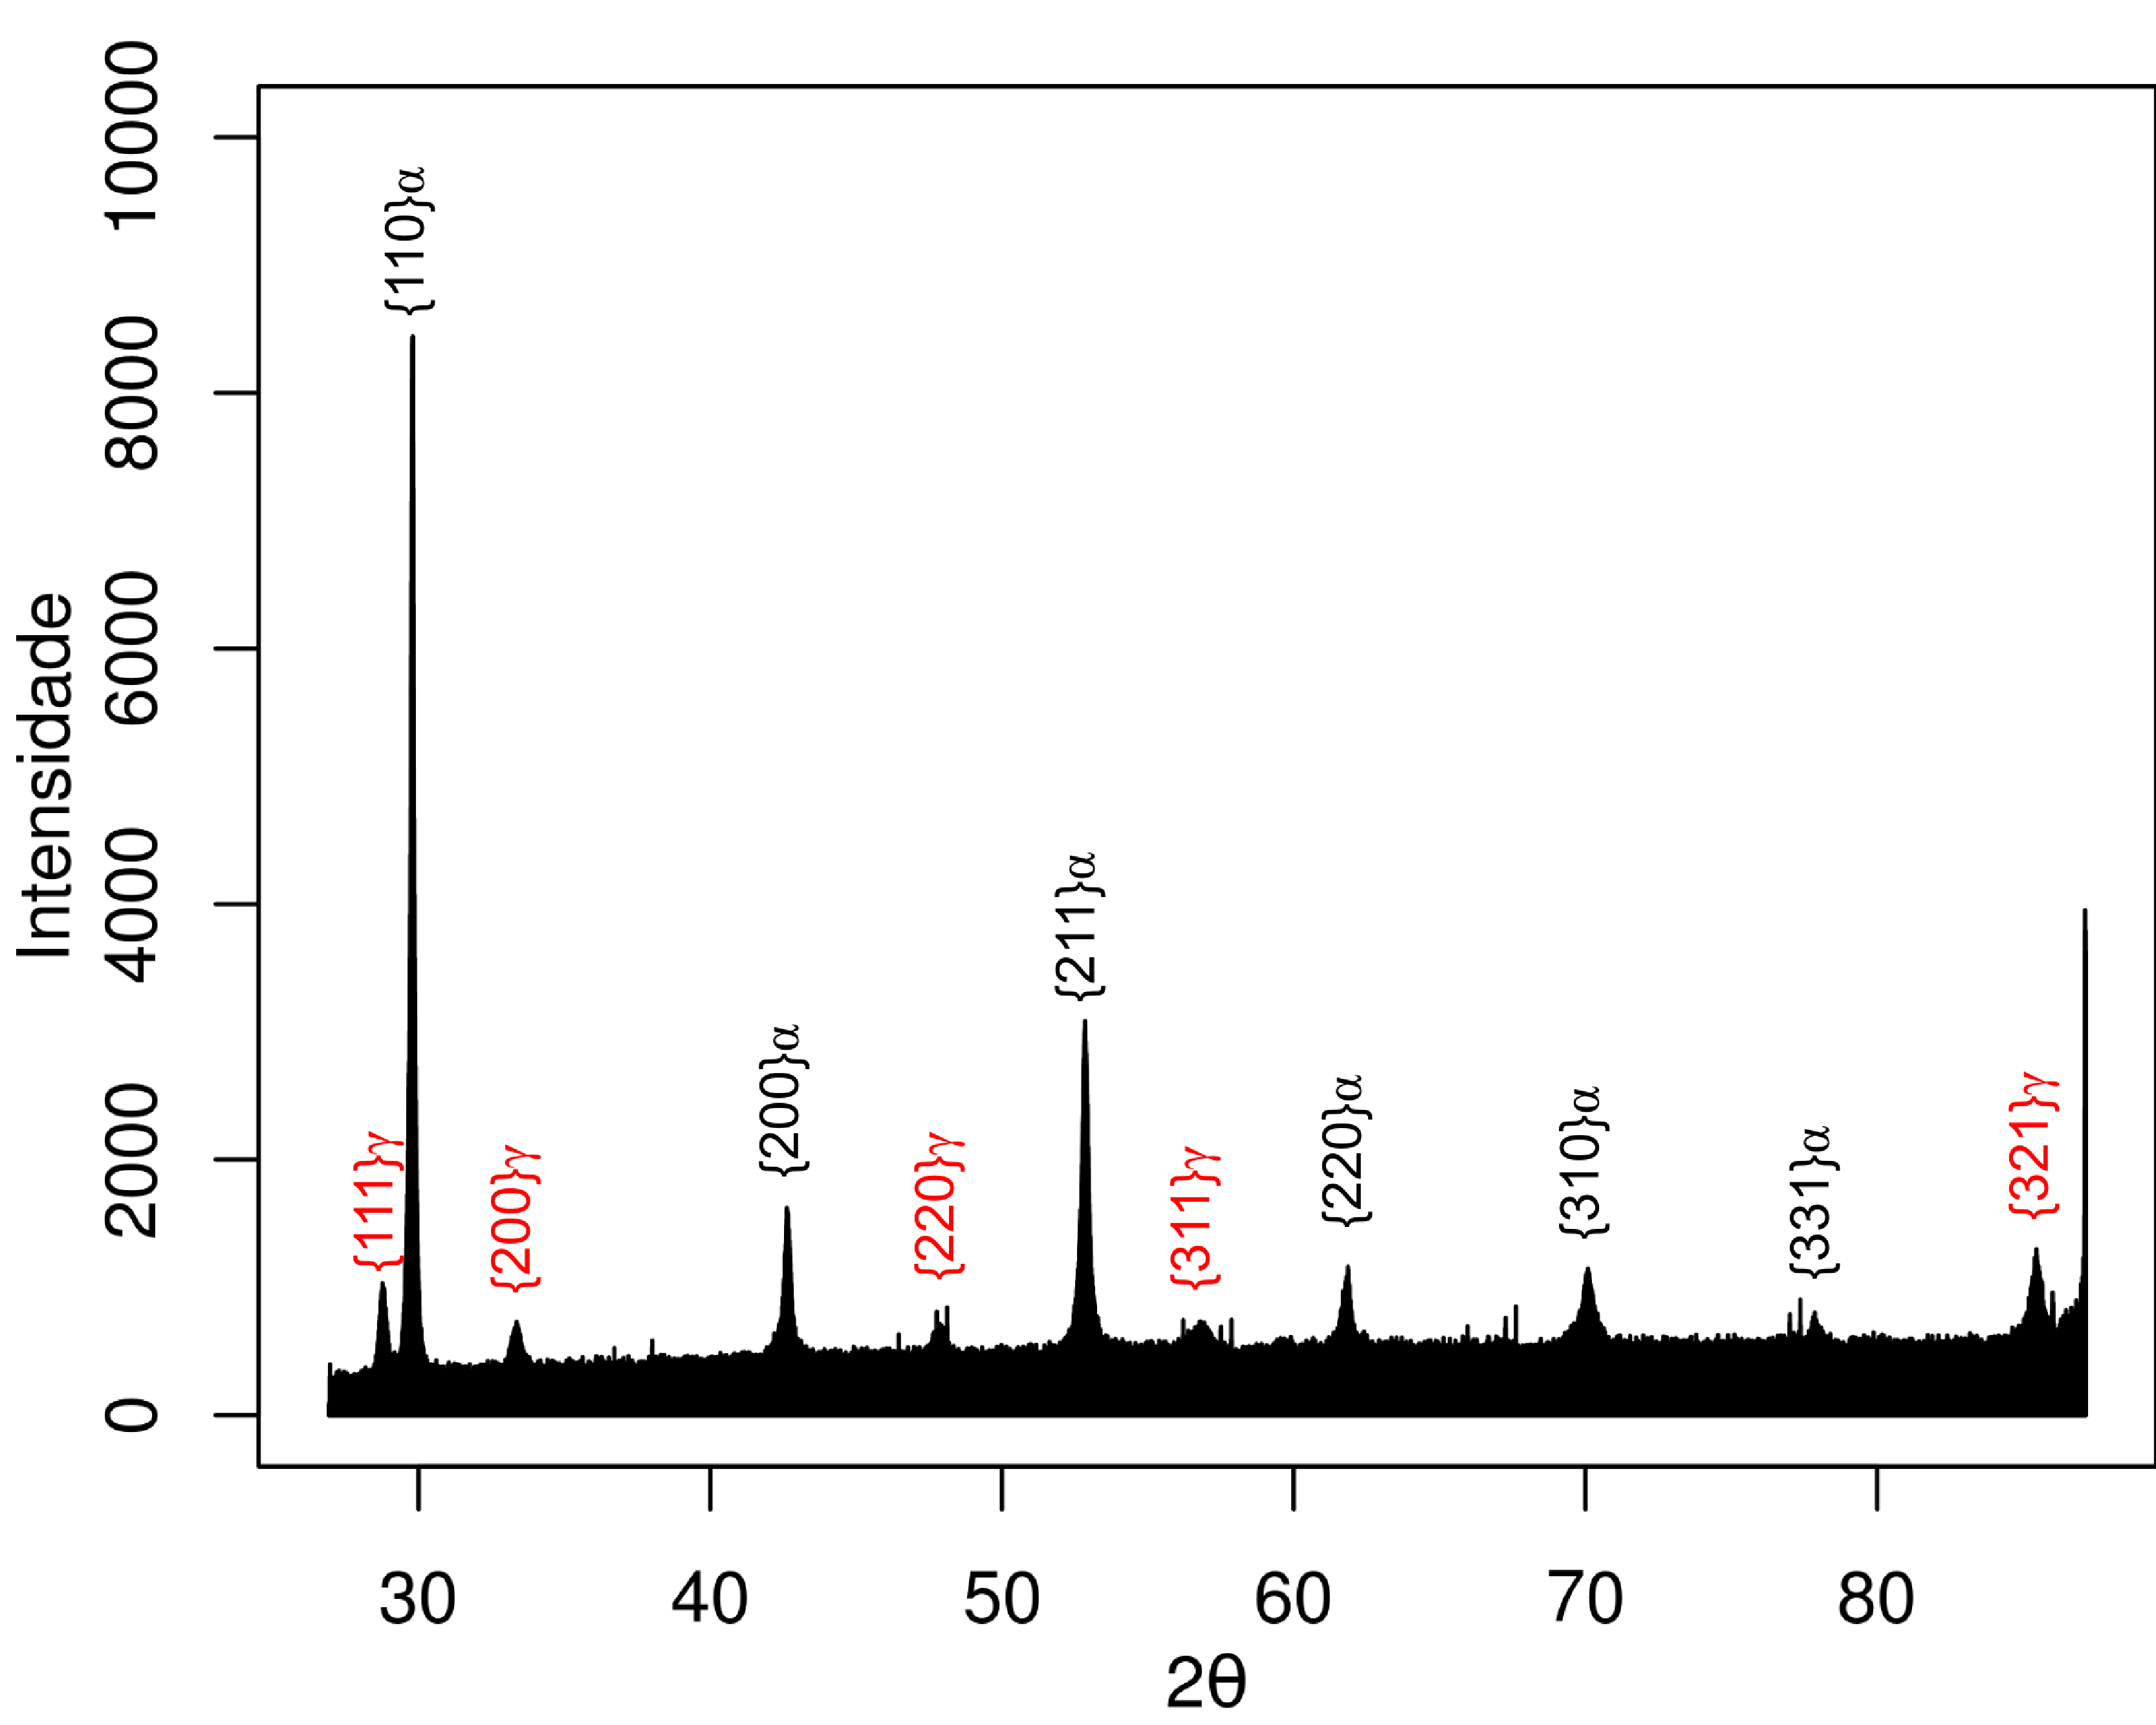
\includegraphics[width=12cm]{img/XTMS/finalScan.png}
	\caption{Difratograma da amostra temperada a 170 °C e particionada a 300 °C obtido pela varredura de $2\theta$ entre 26 e 86°.}
	\label{fig:finalScan}
\end{figure}

\begin{table}
	\caption{Frações volumétricas de austenita retida ($f^\gamma$) e variações nas porcentagens de carbono dissolvidas na austenita ($\Delta w_C^\gamma$) após o processo T\&P para cada condição estudada.}
	\begin{tabular}{c c c c ' c c c c}
	\thickhline
	TT [°C] & TP [°C] & $f^\gamma$ & $\Delta \%w_C^\gamma$ & TT [°C] & TP [°C] & $f^\gamma$ & $\Delta \%w_C^\gamma$\\
	\hline
	140 & 200 & 0,22 & 0,01 & 140 & 375 & 0,16 & 0,57\\
	170 & 200 & 0,20 & 0,01 & 170 & 375 & 0,23 & 0,71\\
	200 & 200 & 0,21 & 0,01 &&&&\\ %200 & 375 & -\\
	\hline
	140 & 250 & 0,22 & 0,13 & 140 & 450 & 0 & -\\
	170 & 250 & 0,23 & 0,10 & 170 & 450 & 0 & -\\
	200 & 250 & 0,27 & 0,06 &&&&\\ %200 & 450 & -\\
	\hline
	140 & 300 & 0,14 & 0,60 &&&&\\
	170 & 300 & 0,15 & 0,62 &&&&\\
	200 & 300 & 0,15 & 0,64 &&&&\\
	\thickhline
	\end{tabular}
	\label{tab:fracGamma}
\end{table}

Como pode ser notado, as condições de partição a 200 e 250 °C produziram as maiores quantidades de austenita retida ao processo T\&P. No entanto, deve ser ressaltado que nessas condições a austenita não atingiu completa estabilidade à temperatura ambiente pela insuficiente partição de carbono. Dessa forma, nessas amostras há significativas quantidades de martensita fresca formada durante o resfriamento final que, por não ter sido submetida a processo subsequente de revenimento, deve conferir caráter frágil ao material.

Como já fora pontuado anteriormente, as amostras particionadas a 450 °C tiveram toda a austenita consumida pela reação isotérmica durante a etapa de partição e, portanto, não apresentam austenita à temperatura ambiente.

As amostras particionadas a 300 e 375 °C foram as únicas que conseguiram reter completamente a austenita enriquecida em carbono durante a etapa de partição. As amostras particionadas a 375 °C apresentaram frações de austenita ligeiramente superiores às encontradas nas amostras particionadas a 300 °C. A condição de têmpera a 170 °C e partição a 375 °C foi a que apresentou maior retenção de austenita.

Em comparação com as estimativas de $\Delta \%w_C^\gamma$ feitas a partir dos resultados de dilatometria (tabela \ref{tab:wCgammaAndrews}), os valores determinados pela dilatometria mostraram-se consistentemente mais elevados. Com efeito, como já discutido, os resultados de DRX mostram variações desprezíveis no carbono dissolvido na austenita durante as etapas de partição a 200 °C. No entanto, considerável diminuição da temperatura Ms foi observada para estas condições nos experimentos de dilatometria. É possível que esta diferença resulta de outros mecanismos de diminuição da temperatura Ms não previstos pela equação de Andrews. Por exemplo, o tamanho dos blocos não transformados de austenita a redistribuição do carbono em seu interior para as discordâncias (formação de atmosferas de Cottrell) poderiam exercer alguma influência sobre a estabilidade da austenita.

Os resultados expostos na tabela \ref{tab:fracGamma} também foram comparados com os valores previstos pelo modelo de equilíbrio restringido de carbono, tal como descrito na seção \ref{subsec:tempOtima}. Na figura \ref{fig:ERCxEXP} a curva sólida representam os valores previstos pelo modelo ERC, construído utilizando como parâmetro de entrada o teor de carbono da austenita calculado pelo software Thermo-Calc\textregistered{} (i.e., 0,76\%). Os dados experimentais são apresentados na forma de pontos superpostos à figura.

\begin{figure}
	\includegraphics[width=12cm]{img/ERCxEXP.png}
	\caption{Comparação da porcentagem de austenita (em volume) prevista com a obtida experimentalmente após a aplicação do processo T\&P.}
	\label{fig:ERCxEXP}
\end{figure}

Nota-se que, com exceção das amostras temperadas a 200 °C, todas as condições apresentaram frações volumétricas de austenita consideravelmente inferiores à previsão do modelo ERC. Isso é provavelmente decorre do fato de que nem todo o potencial de partição de carbono foi atingido após o tratamento térmico em função da não-eliminação da supersaturação do carbono da austenita, ou pela precipitação de carbonetos do revenimento, como pontuado na seção \ref{subsec:wCalpha}.